\chapter{Results}
\label{chapter7}

In this chapter we will exhibit some screenshots of the main screens of NokScanner, detailing the most relevant elements of the user interface and introducing the final design of the mobile application. We will also present some practical use cases in order to test the accuracy of the app.

\section{Device specifications}

This section details the main characteristics of the testing device used to verify the adequate working of the mobile application, to be taken as reference in case of any possible issues that may arise when using the app on other devices.

During the development of this project, the only device available for testing was the author personal Android device. Therefore, this app has not been tested on an iOS device (iPhone, iPad, etc.) and may not work on one without further troubleshooting, which could be explored and developed as future work. The specifications of the device used are the following:

\begin{itemize}
\item \textbf{Device model}: Samsung A51 5G
\item \textbf{Operative system}: Android 11
\item \textbf{Processsor}: Samsung Exynos 980 (Octa-core, 2x 2.2GHz + 6x 1.8GHz, 64-bit)
\item \textbf{Internal memory}: 6 GB RAM
\item \textbf{Storage memory}: 128 GB
\item \textbf{Screen}: 6.5 inches, 2400 x 1080 pixels
\item \textbf{Camera}: 48MP quad camera (back), 32MP camera (front)
\end{itemize}

\section{User interface}

Below are presented several screenshots of the mobile app showcasing the different screens and components of the user interface.

\subsection{History}

This is the screen loaded when starting the app. An empty history shows a prompt to try to scan for the first time (Figure \ref{fig:history-empty}). After some scans, the history shows the recent entries sorted by date, also displaying their name and image (Figure \ref{fig:history}).

\begin{figure}[h]
    \begin{subfigure}{0.5\textwidth}
        \centering
        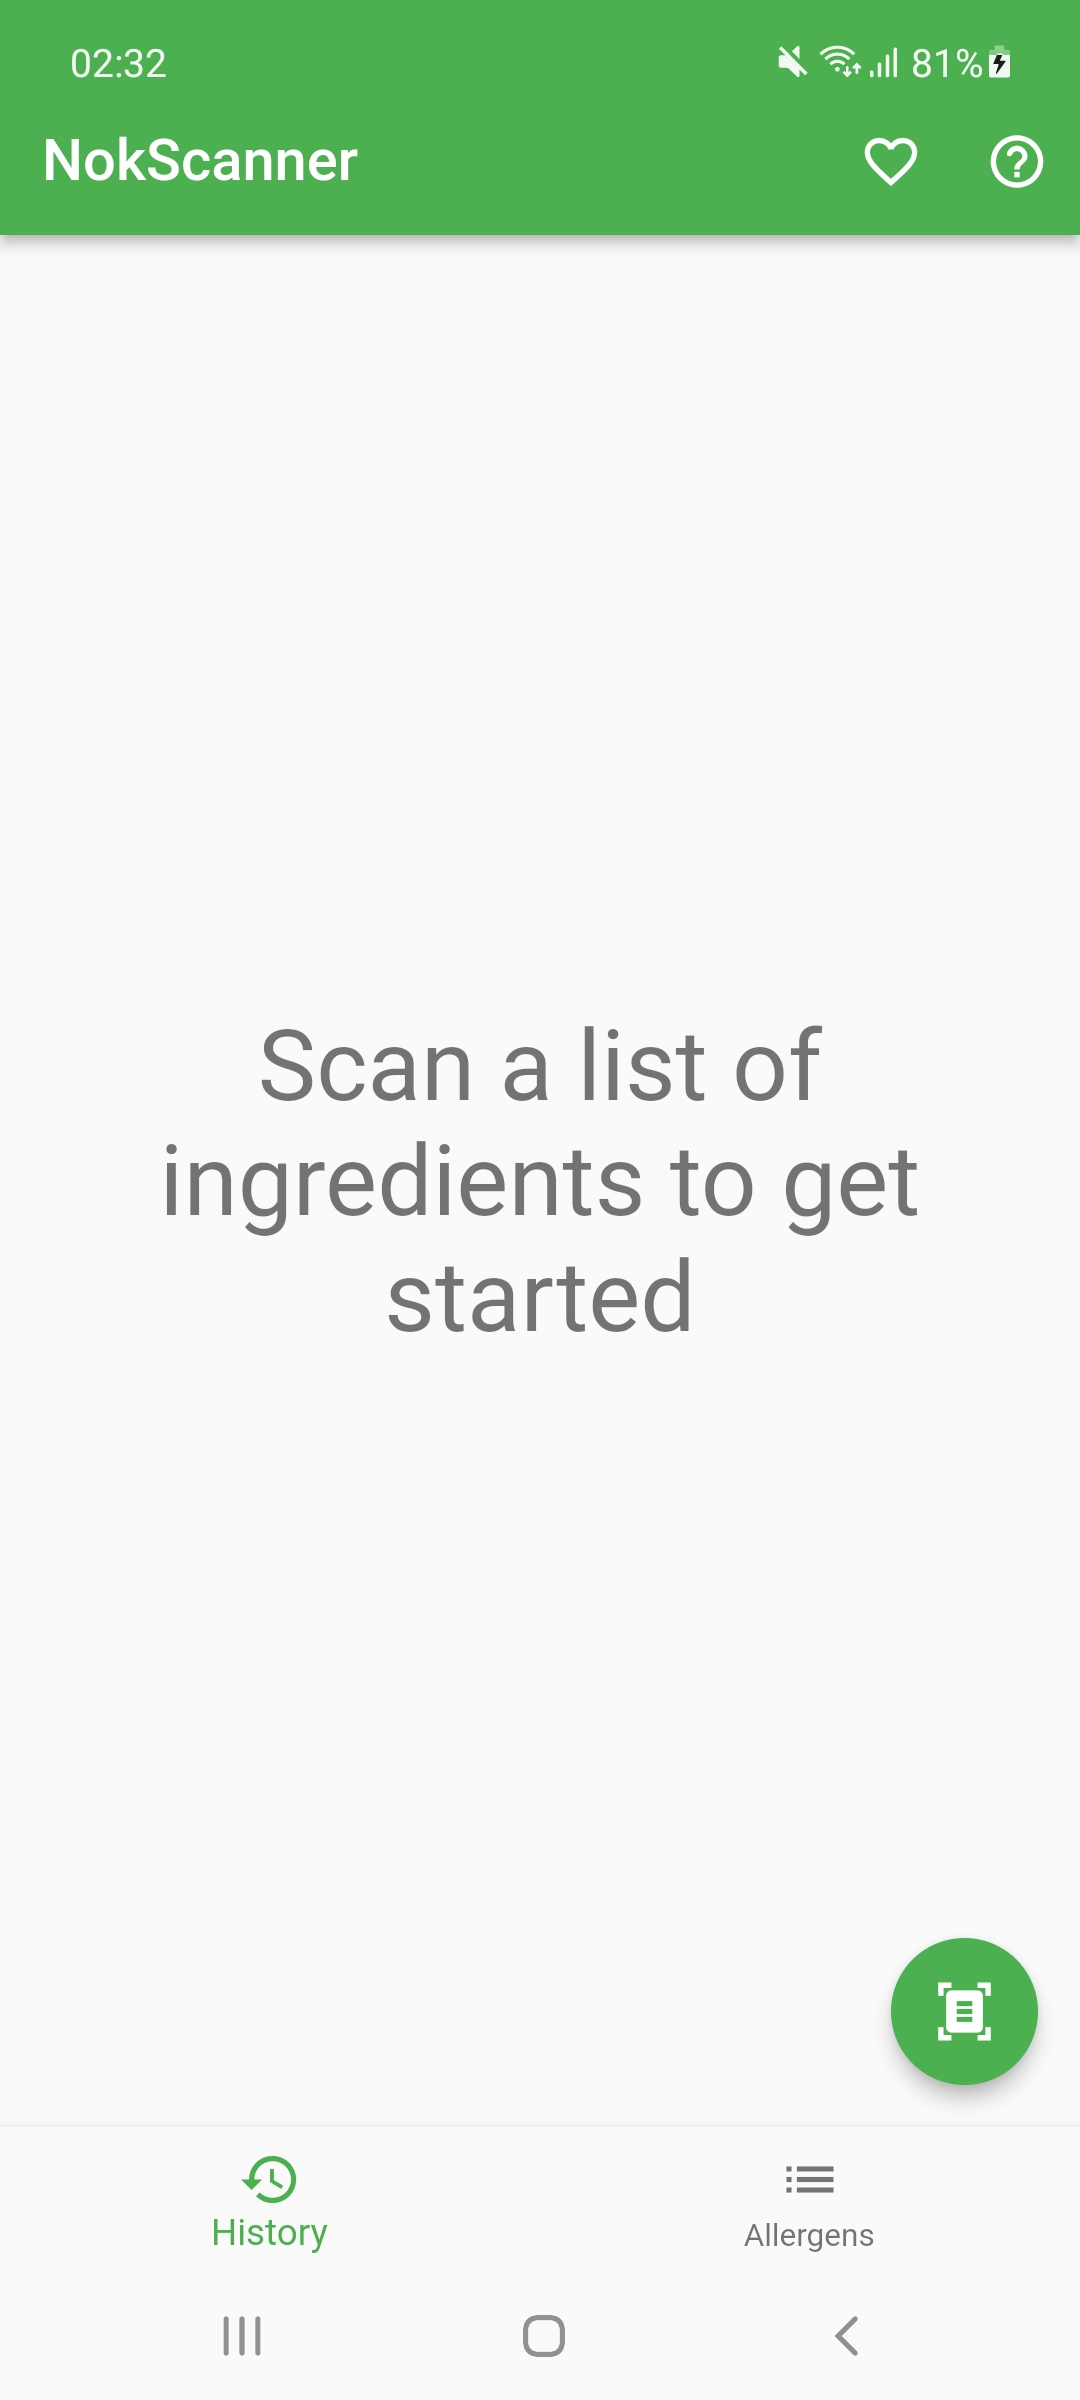
\includegraphics[width=0.9\linewidth]{Figures/Screenshot/history_empty.jpg} 
        \caption{Empty history}
        \label{fig:history-empty}
    \end{subfigure}
    \begin{subfigure}{0.5\textwidth}
        \centering
        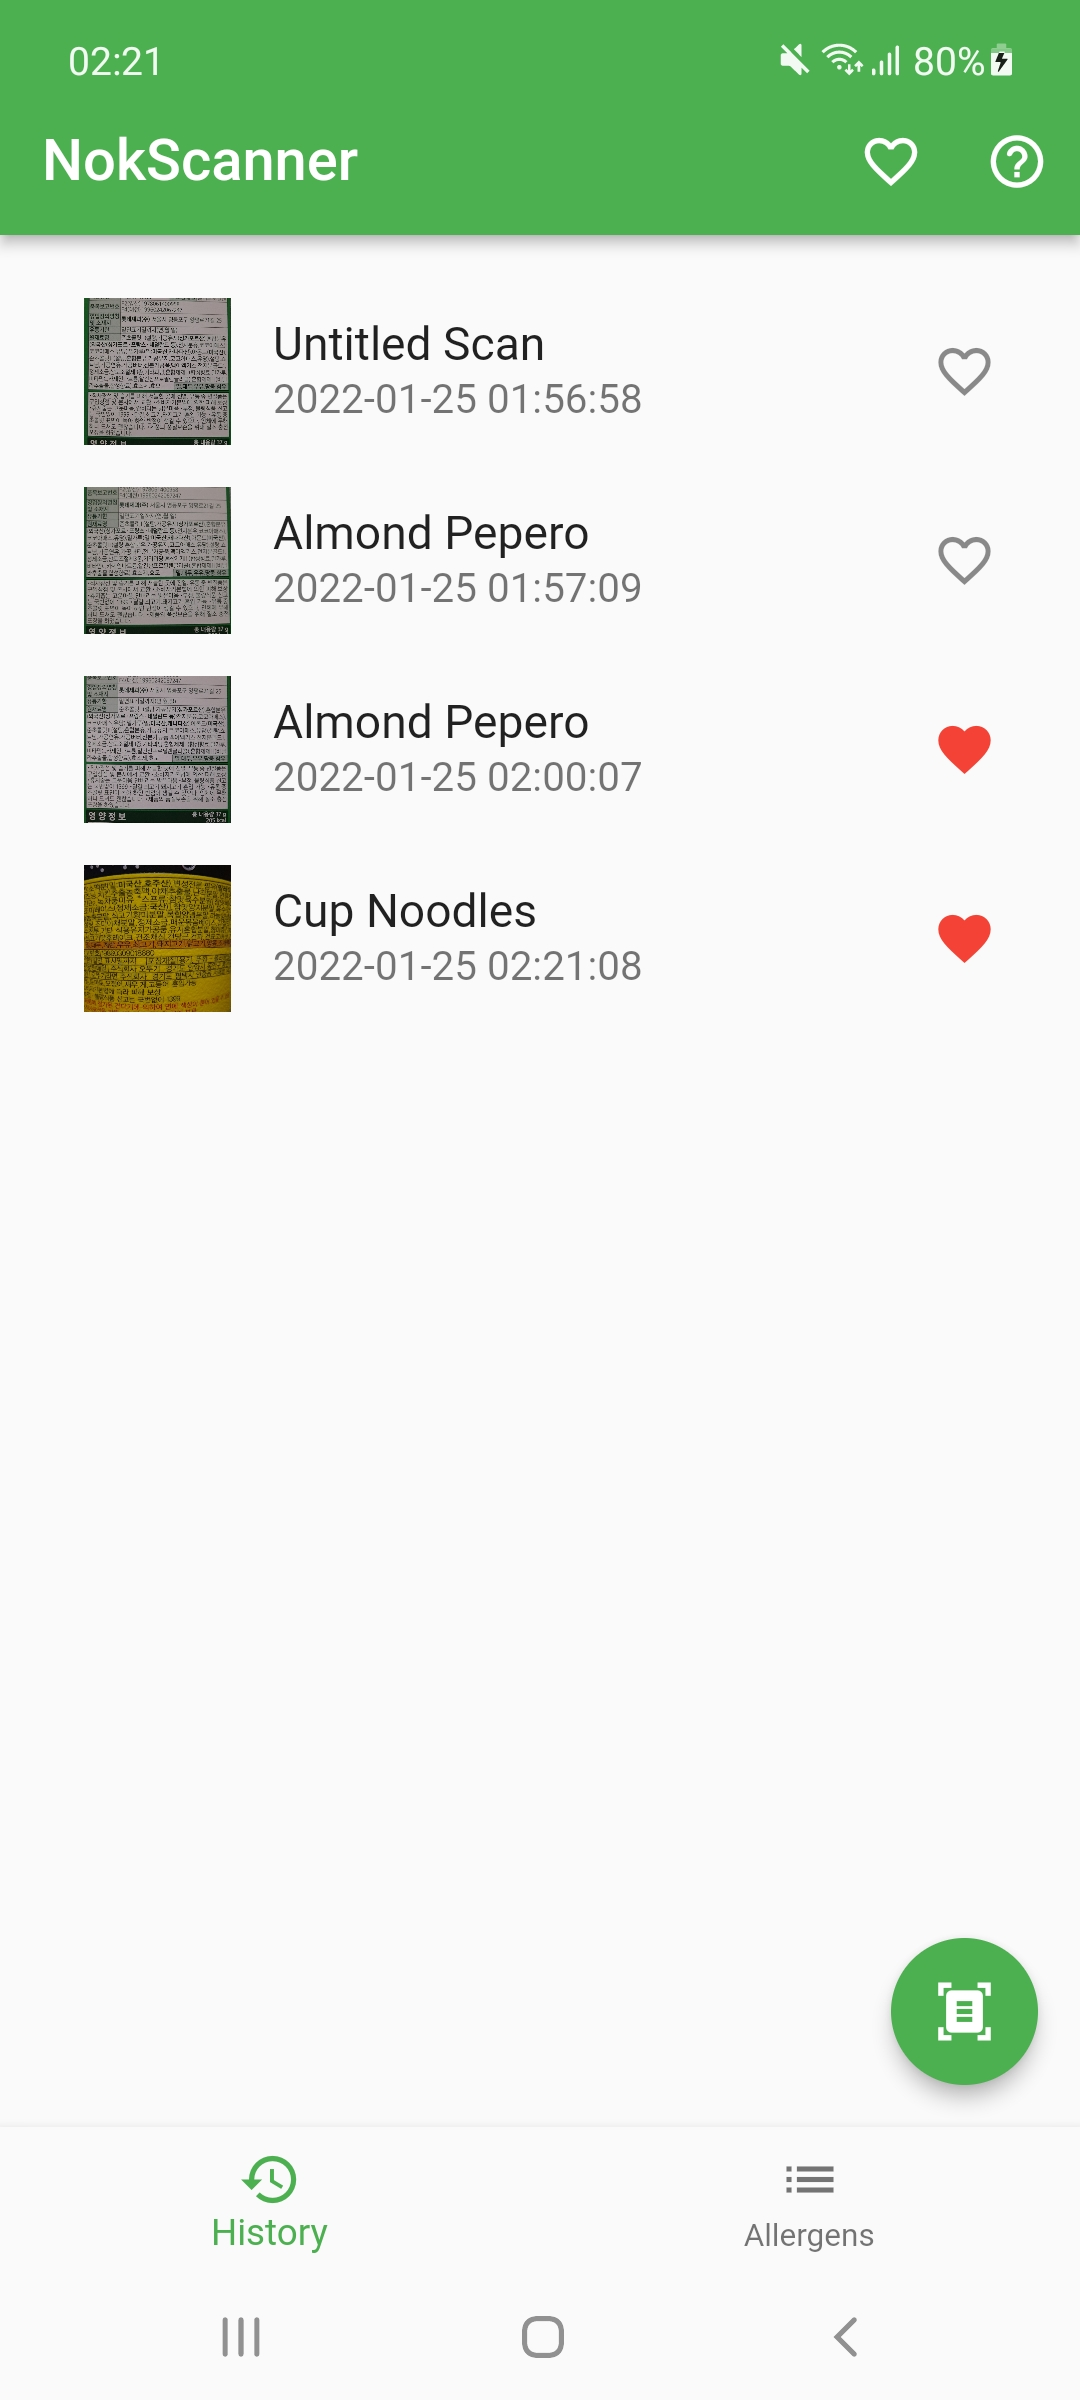
\includegraphics[width=0.9\linewidth]{Figures/Screenshot/history.jpg}
        \caption{Populated history}
        \label{fig:history}
    \end{subfigure}
    \caption{History screen}
    \label{fig:history2}
\end{figure}

By tapping the heart icon, the user can also save some of this entries and keep them inside a dedicated "favorites" view (Figure \ref{fig:favs}). This view is accessed by clicking the heart outline icon on the app bar.

\begin{figure}[h]
  \centering
  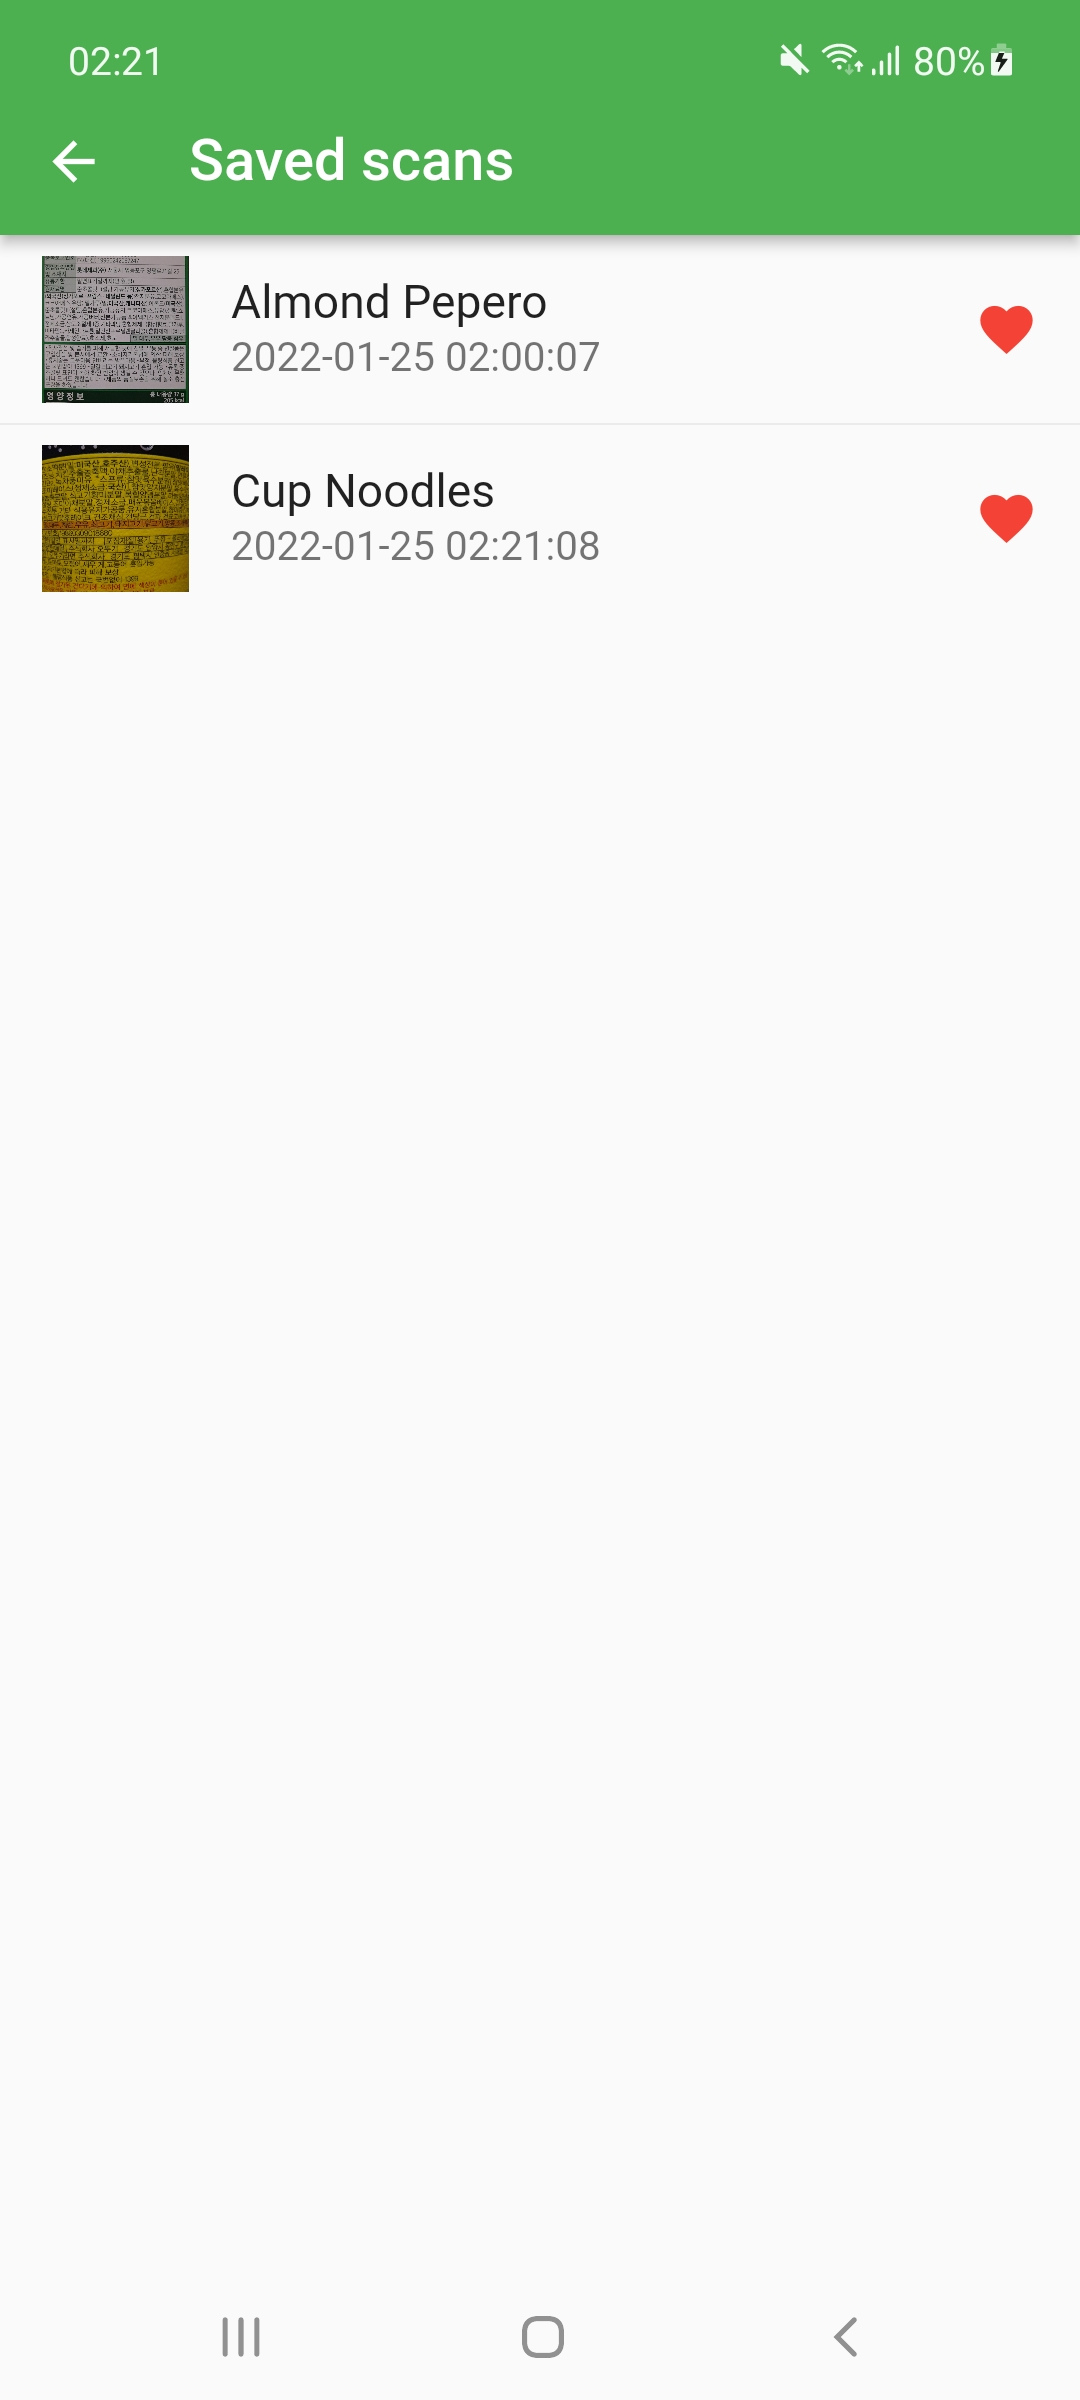
\includegraphics[width=0.5\textwidth]{Figures/Screenshot/favs.jpg}
  \caption{%
    Favorites screen
  }
  \label{fig:favs}
\end{figure}

\clearpage

\subsection{Help and FAQ}

The help screen can be accessed through almost all of the screens in the app through a question mark button at the top right. This screen has 3 panels (Figure \ref{fig:help-collapse}) that can be expanded to show some information about the correct usage of the app and some precautions and safety disclaimers for the user (Figure \ref{fig:help}).

\begin{figure}[h]
    \begin{subfigure}{0.5\textwidth}
        \centering
        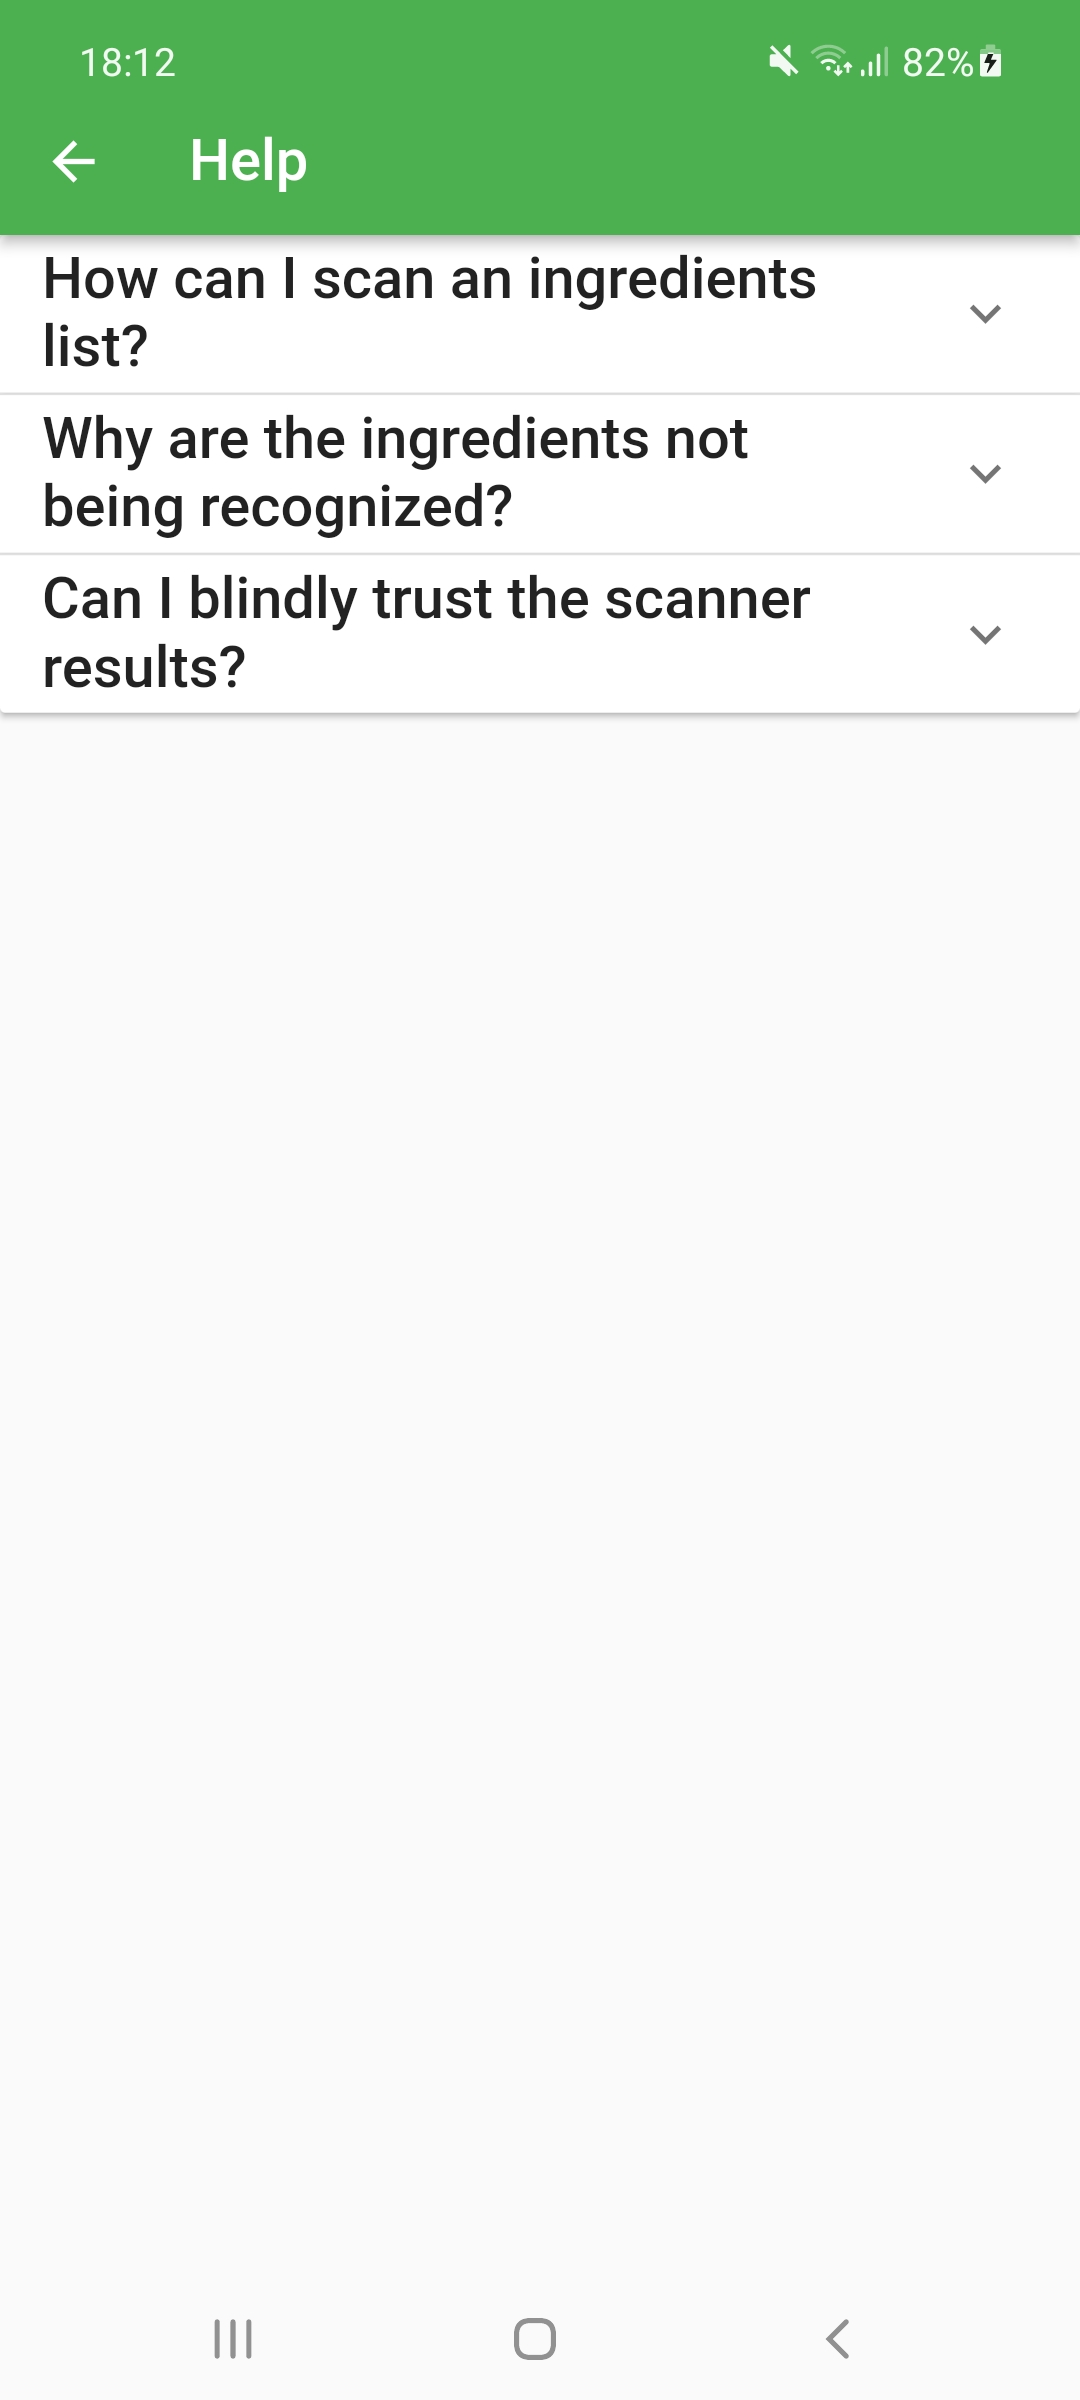
\includegraphics[width=0.9\linewidth]{Figures/Screenshot/help_collapse.jpg} 
        \caption{Collapsed panels}
        \label{fig:help-collapse}
    \end{subfigure}
    \begin{subfigure}{0.5\textwidth}
        \centering
        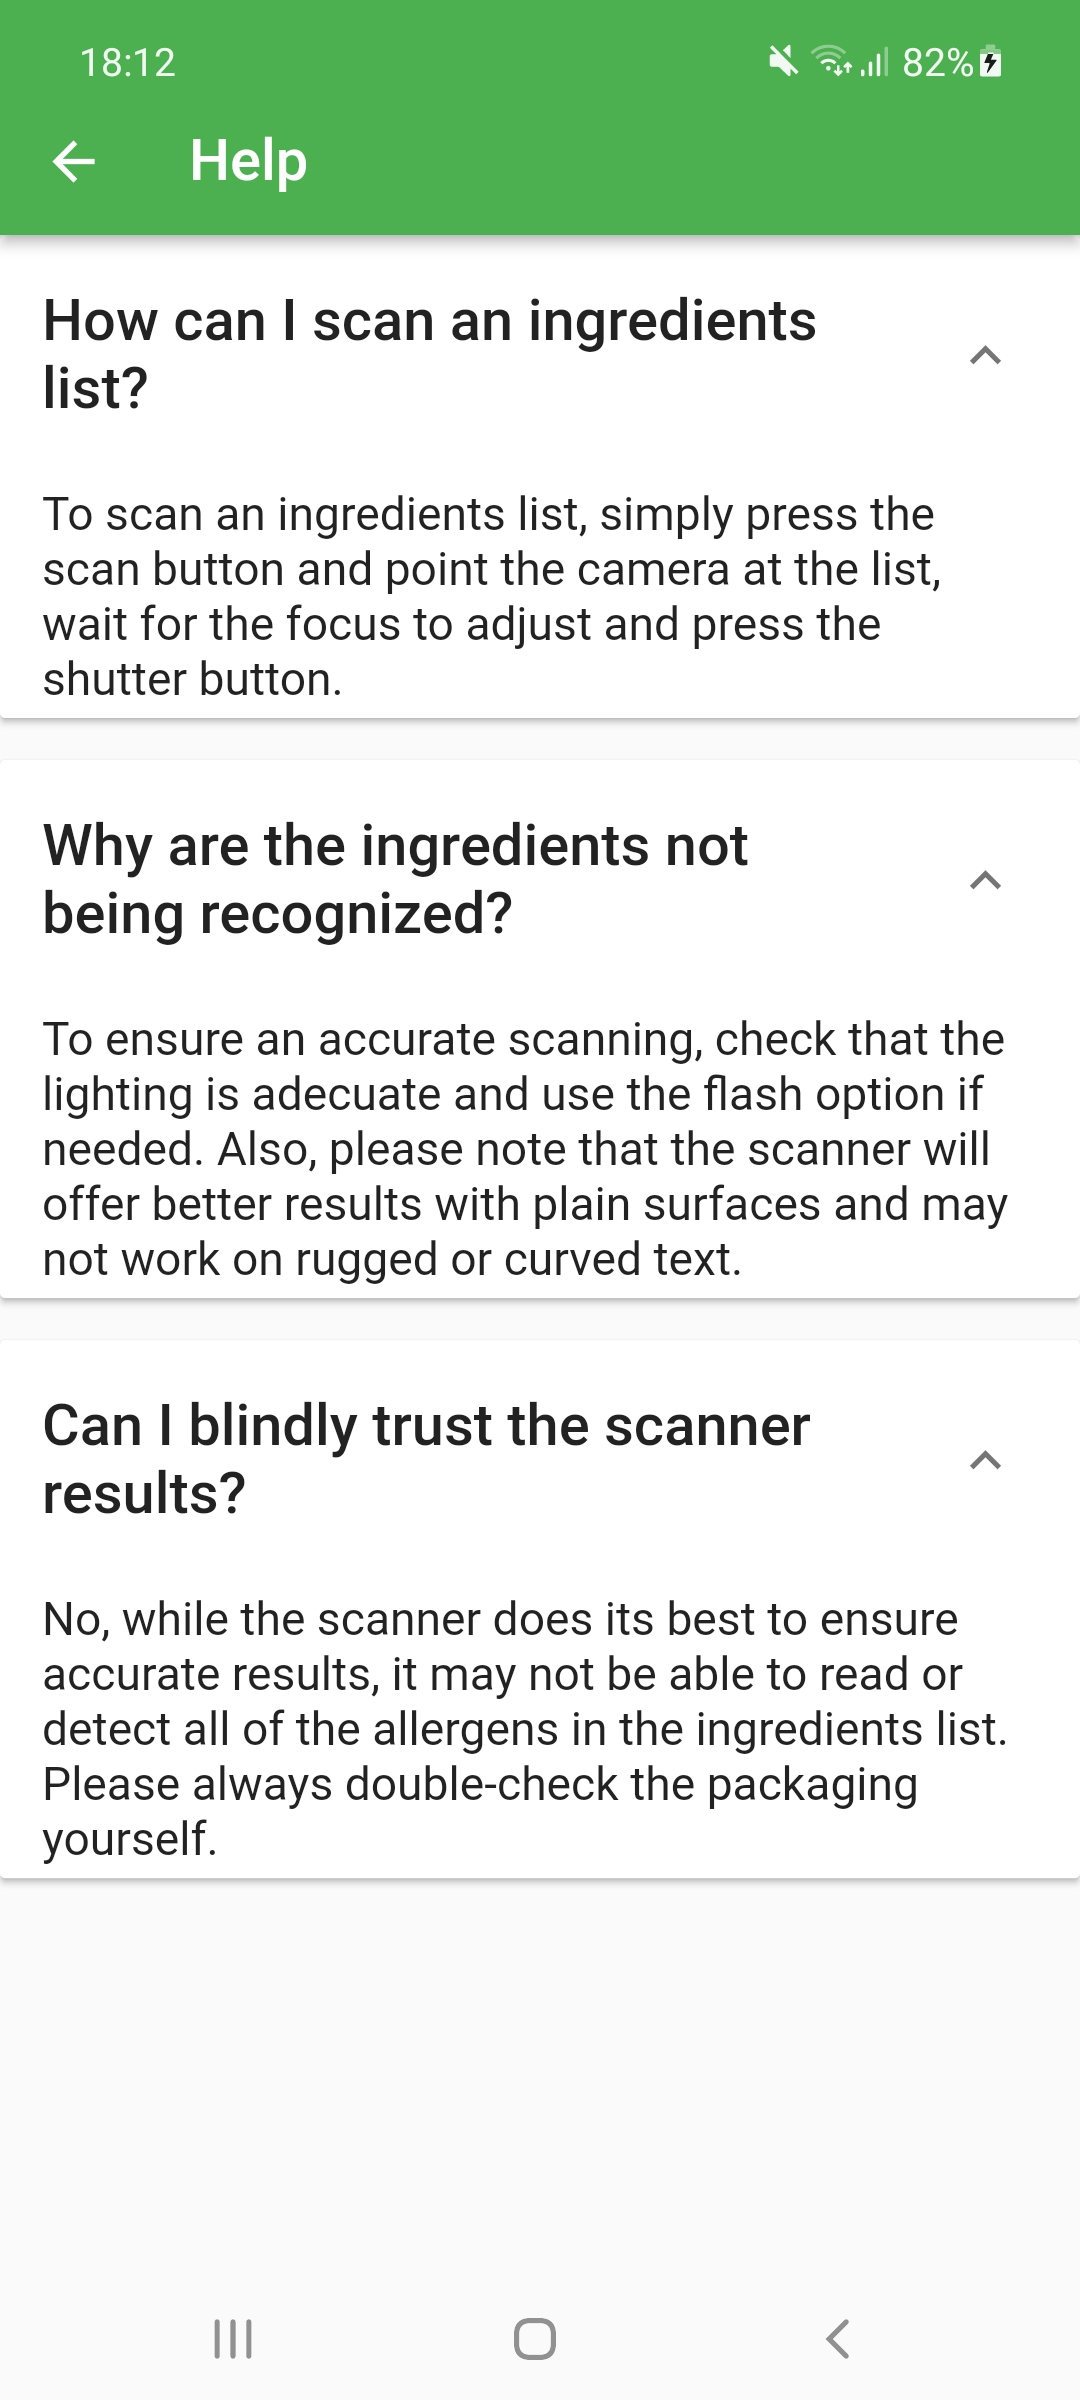
\includegraphics[width=0.9\linewidth]{Figures/Screenshot/help.jpg}
        \caption{Expanded panels}
        \label{fig:help}
    \end{subfigure}
    \caption{Help screen}
    \label{fig:help2}
\end{figure}

\clearpage

\subsection{Camera and gallery}

By tapping the scanner button on the main screen, the user is taken to the camera or scanner view (Figure \ref{fig:camera}). This screen is composed of a full-screen camera preview, a button to take the picture, and action buttons on the top bar to toggle the flash, go to the help view or select a previous photo from the image picker (Figure \ref{fig:image-picker}). This image picker is an Android native element, and upon choosing a picture the user is taken to the results view.

\begin{figure}[h]
    \begin{subfigure}{0.5\textwidth}
        \centering
        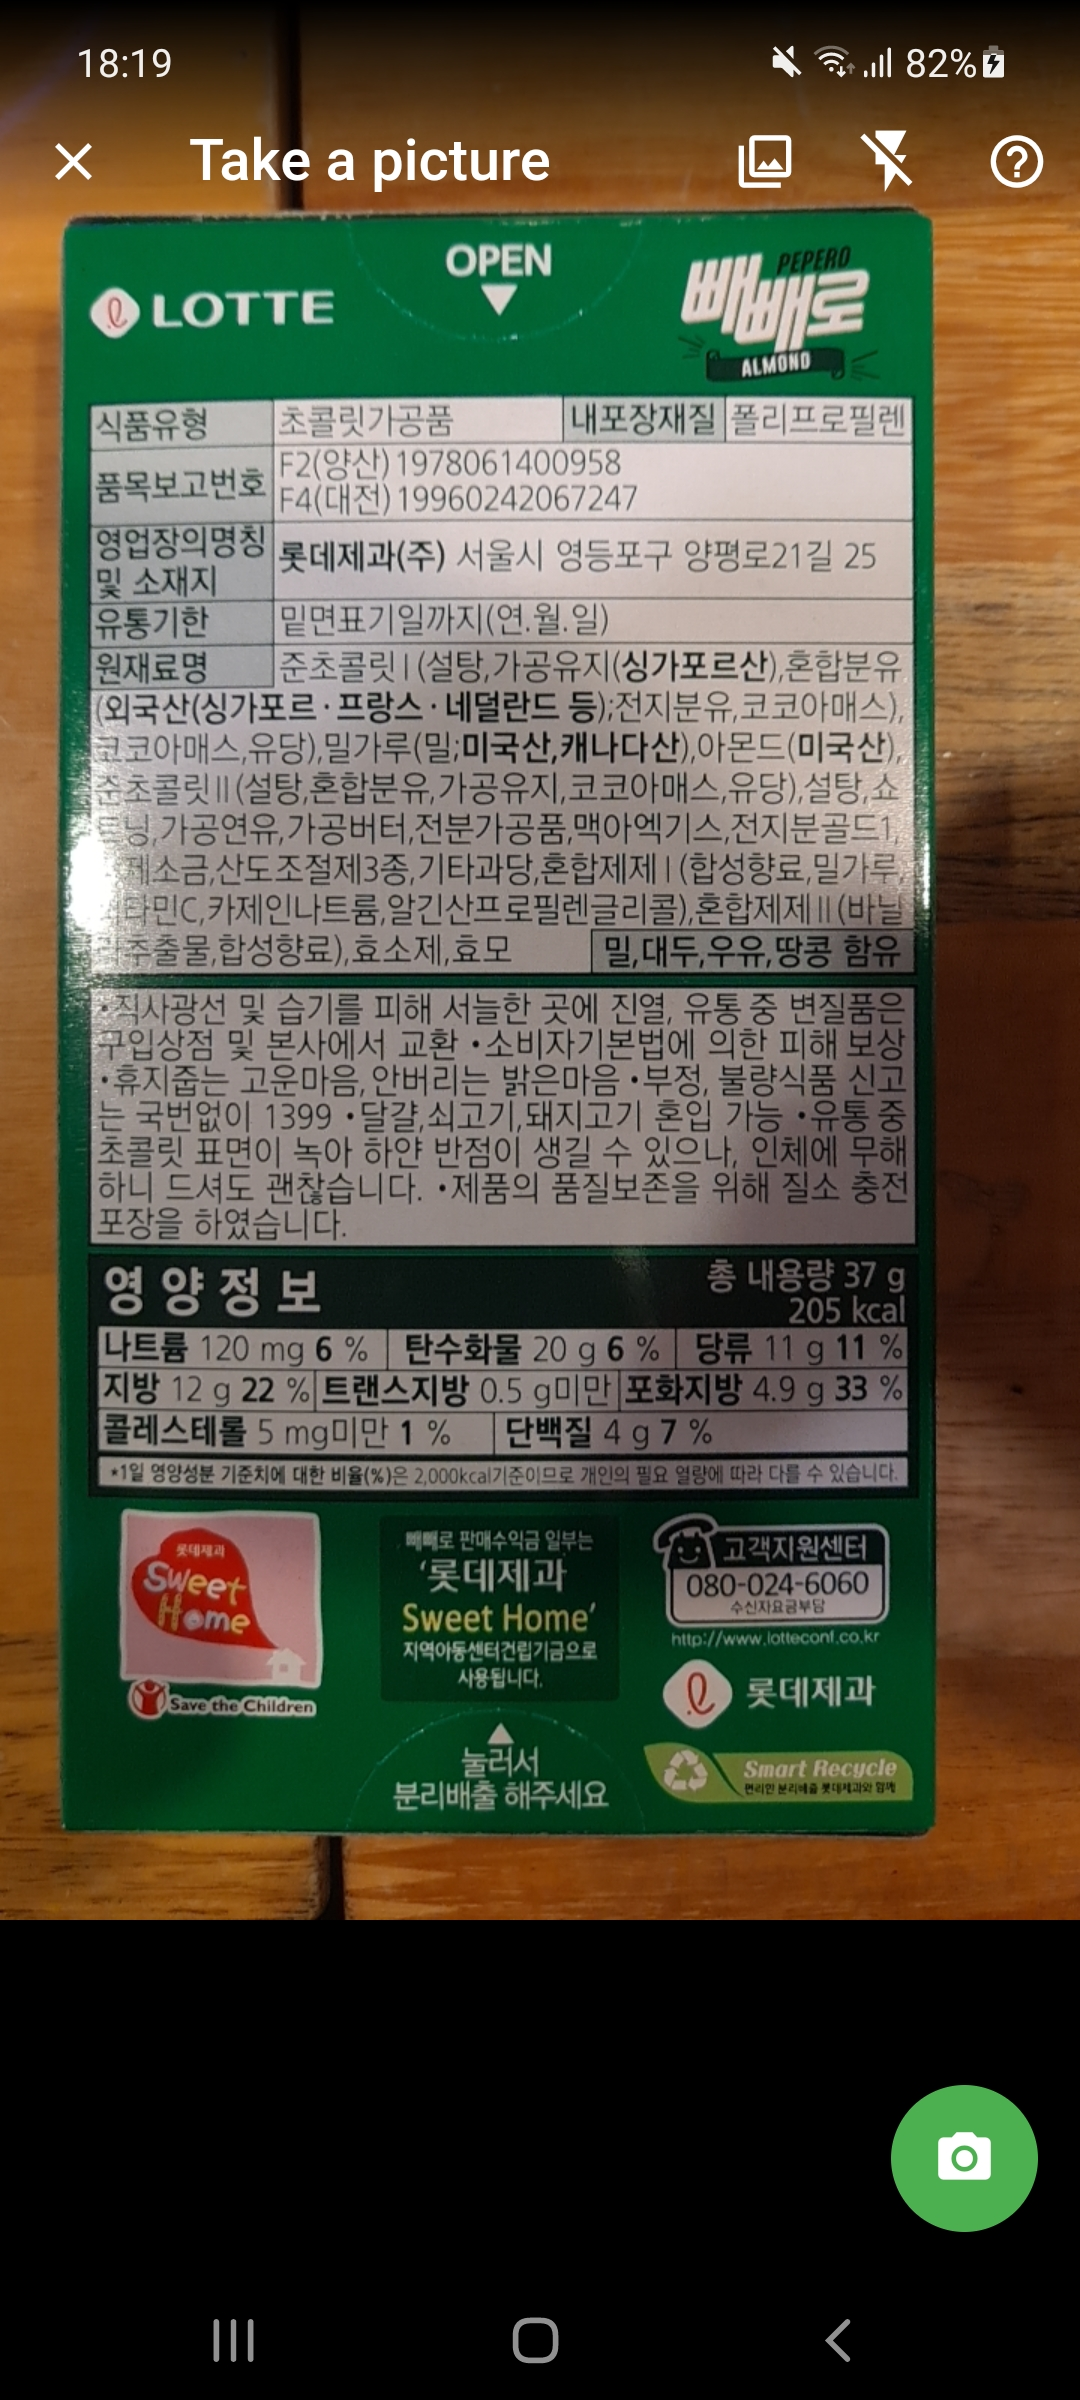
\includegraphics[width=0.9\linewidth]{Figures/Screenshot/camera.jpg} 
        \caption{Camera}
        \label{fig:camera}
    \end{subfigure}
    \begin{subfigure}{0.5\textwidth}
        \centering
        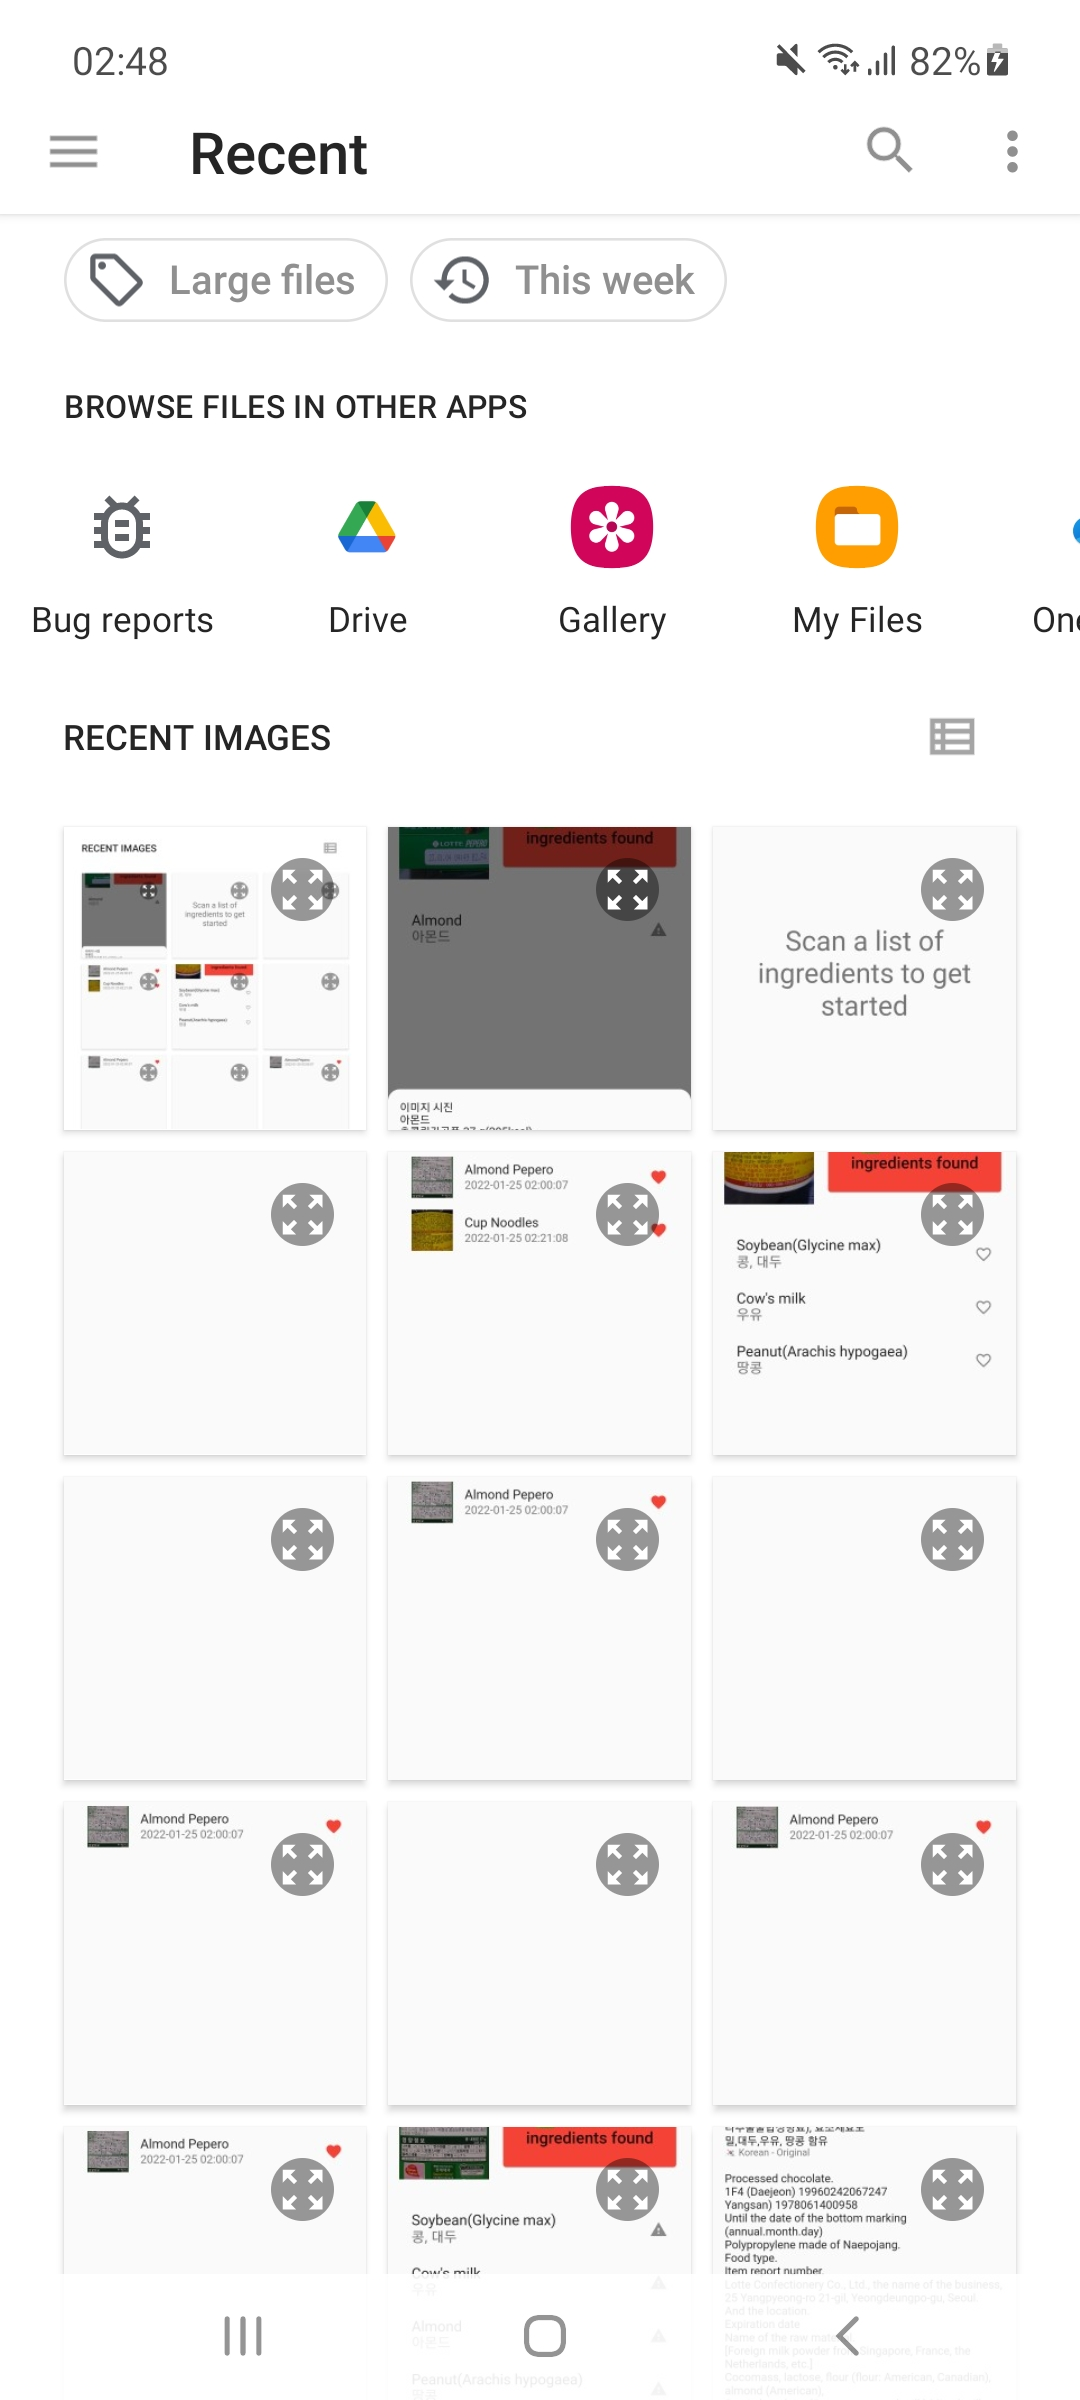
\includegraphics[width=0.9\linewidth]{Figures/Screenshot/image_picker.jpg}
        \caption{Image picker}
        \label{fig:image-picker}
    \end{subfigure}
    \caption{Camera and image picker screens}
    \label{fig:camera2}
\end{figure}

\clearpage

\subsection{Scanning results}

The scanning results screen is composed of a small thumbnail of the image taken, which can be tapped to expand it to full screen, an editable field to input the title that will show on the history, the date and time, and a distinct banner showing the number of unwanted ingredients found. Below this elements, there is either a list of all the unwanted ingredients found in the packaging along with their Korean names (Figure \ref{fig:scan-warn}), or a "no matches found" text along with a disclaimer to double-check manually (Figure \ref{fig:scan-pass}).

\begin{figure}[h]
    \begin{subfigure}{0.5\textwidth}
        \centering
        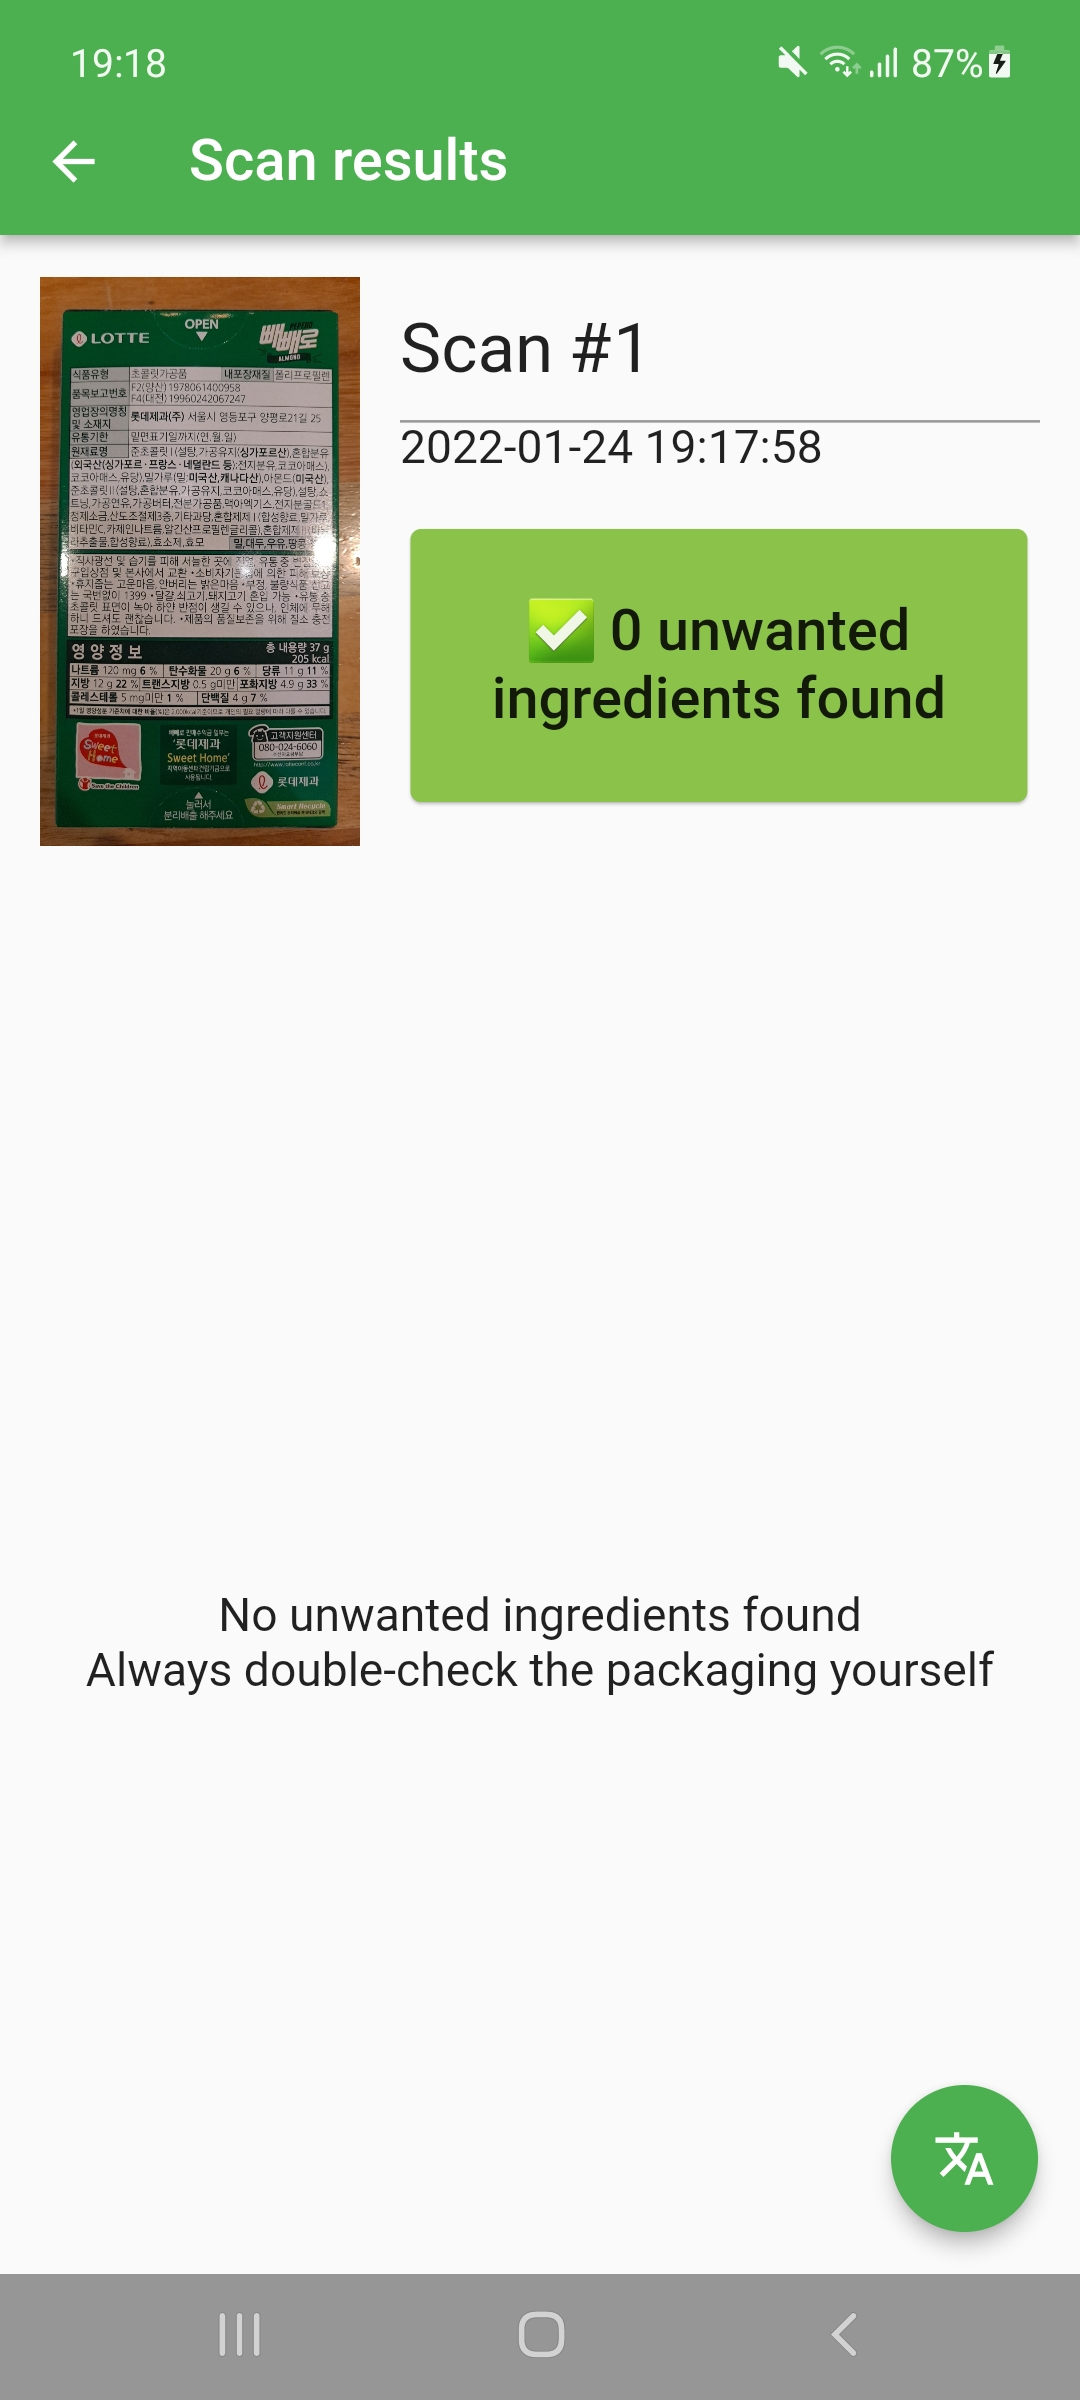
\includegraphics[width=0.9\linewidth]{Figures/Screenshot/scan_pass.jpg} 
        \caption{No unwanted ingredients}
        \label{fig:scan-pass}
    \end{subfigure}
    \begin{subfigure}{0.5\textwidth}
        \centering
        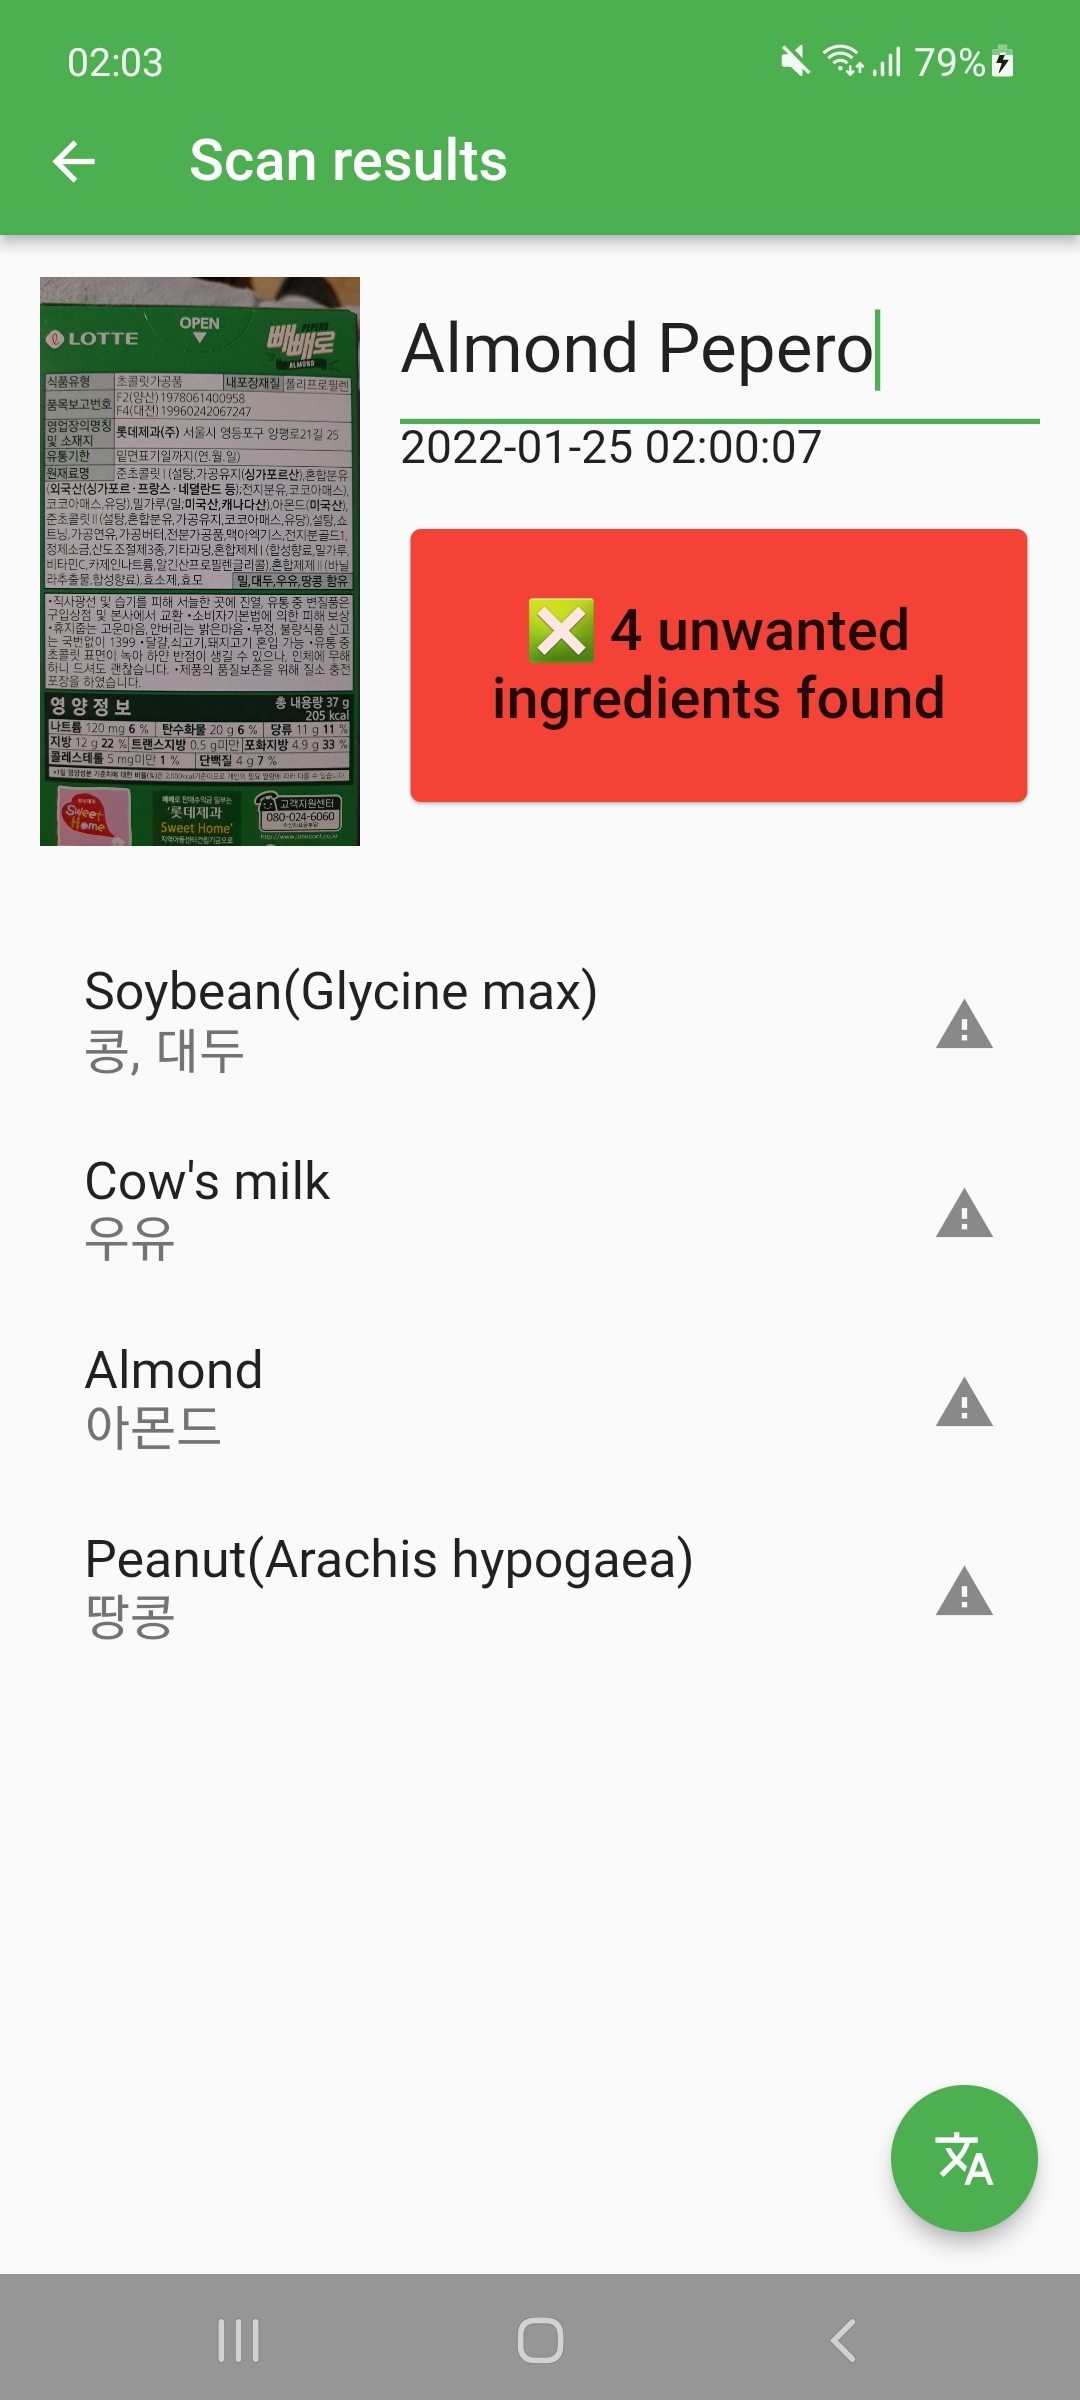
\includegraphics[width=0.9\linewidth]{Figures/Screenshot/scan_warn.jpg}
        \caption{4 unwanted ingredients}
        \label{fig:scan-warn}
    \end{subfigure}
    \caption{Scanning results screen}
    \label{fig:scan}
\end{figure}

\clearpage

\subsection{Text translation}

If the user taps the bottom right icon of the scan results screen, a modal sheet will pop up displaying both the recognized text in Korean as well as the translated text in English (Figure \ref{fig:translate}). This way the user can manually double-check if they suspect a synonym for an unwanted ingredient may have been left unrecognized by the application.

\begin{figure}[h]
  \centering
  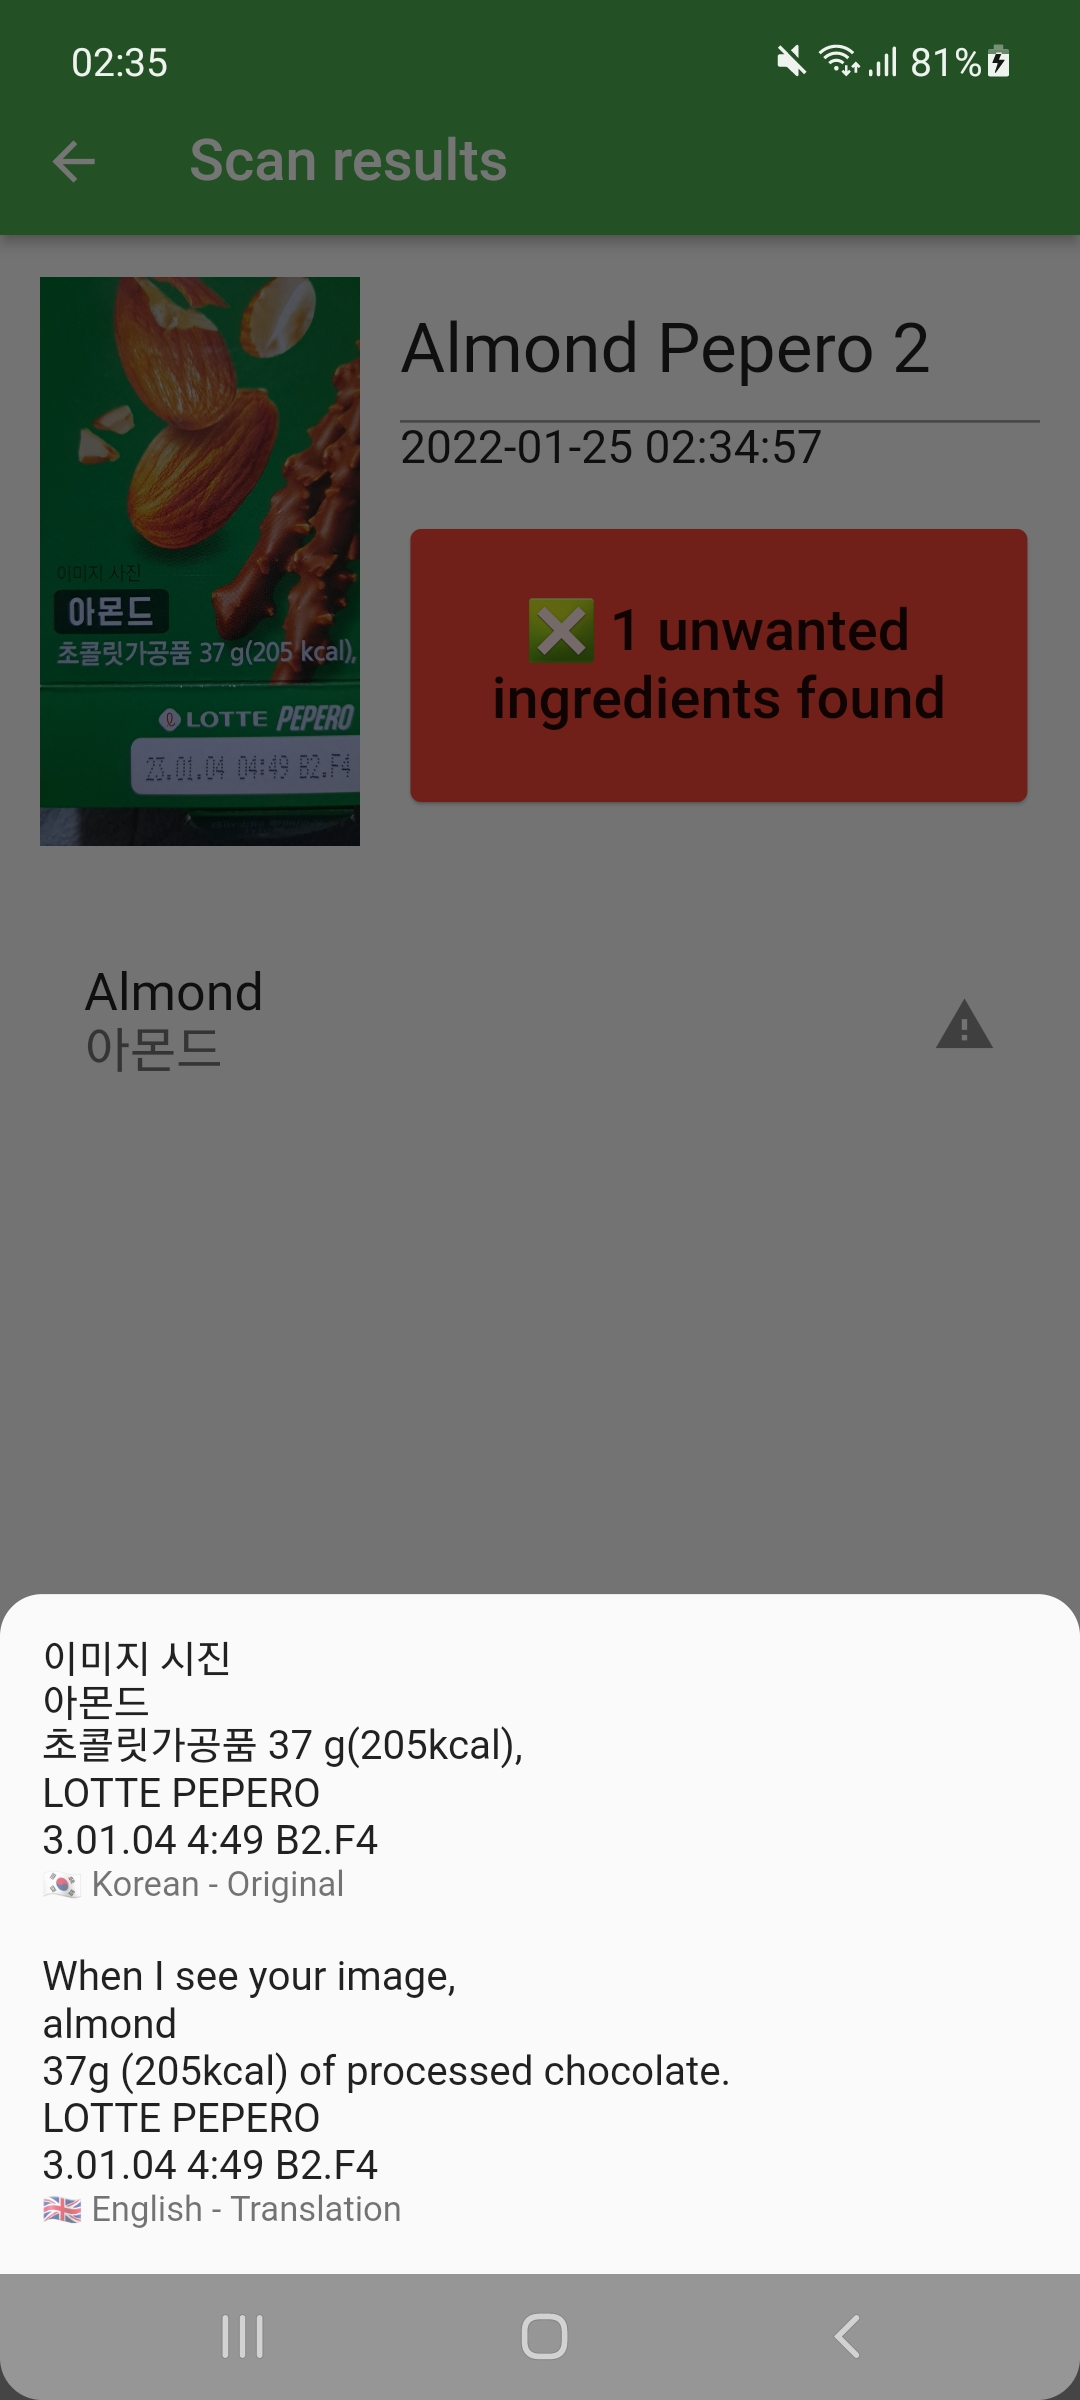
\includegraphics[width=0.5\textwidth]{Figures/Screenshot/papago.jpg}
  \caption{%
    Translation modal sheet
  }
  \label{fig:translate}
\end{figure}

\clearpage

\subsection{Allergens}

In the allergens view, the user can see all of the active filters or ingredients to be detected by the app when running a scan (Figure \ref{fig:ingredients}). Every entry is shown with both the names in English and Korean, and they can be disabled at any moment by clicking the trash can icon to the right. The user can add more of these filters at any time by tapping the add (+) button.

\begin{figure}[h]
  \centering
  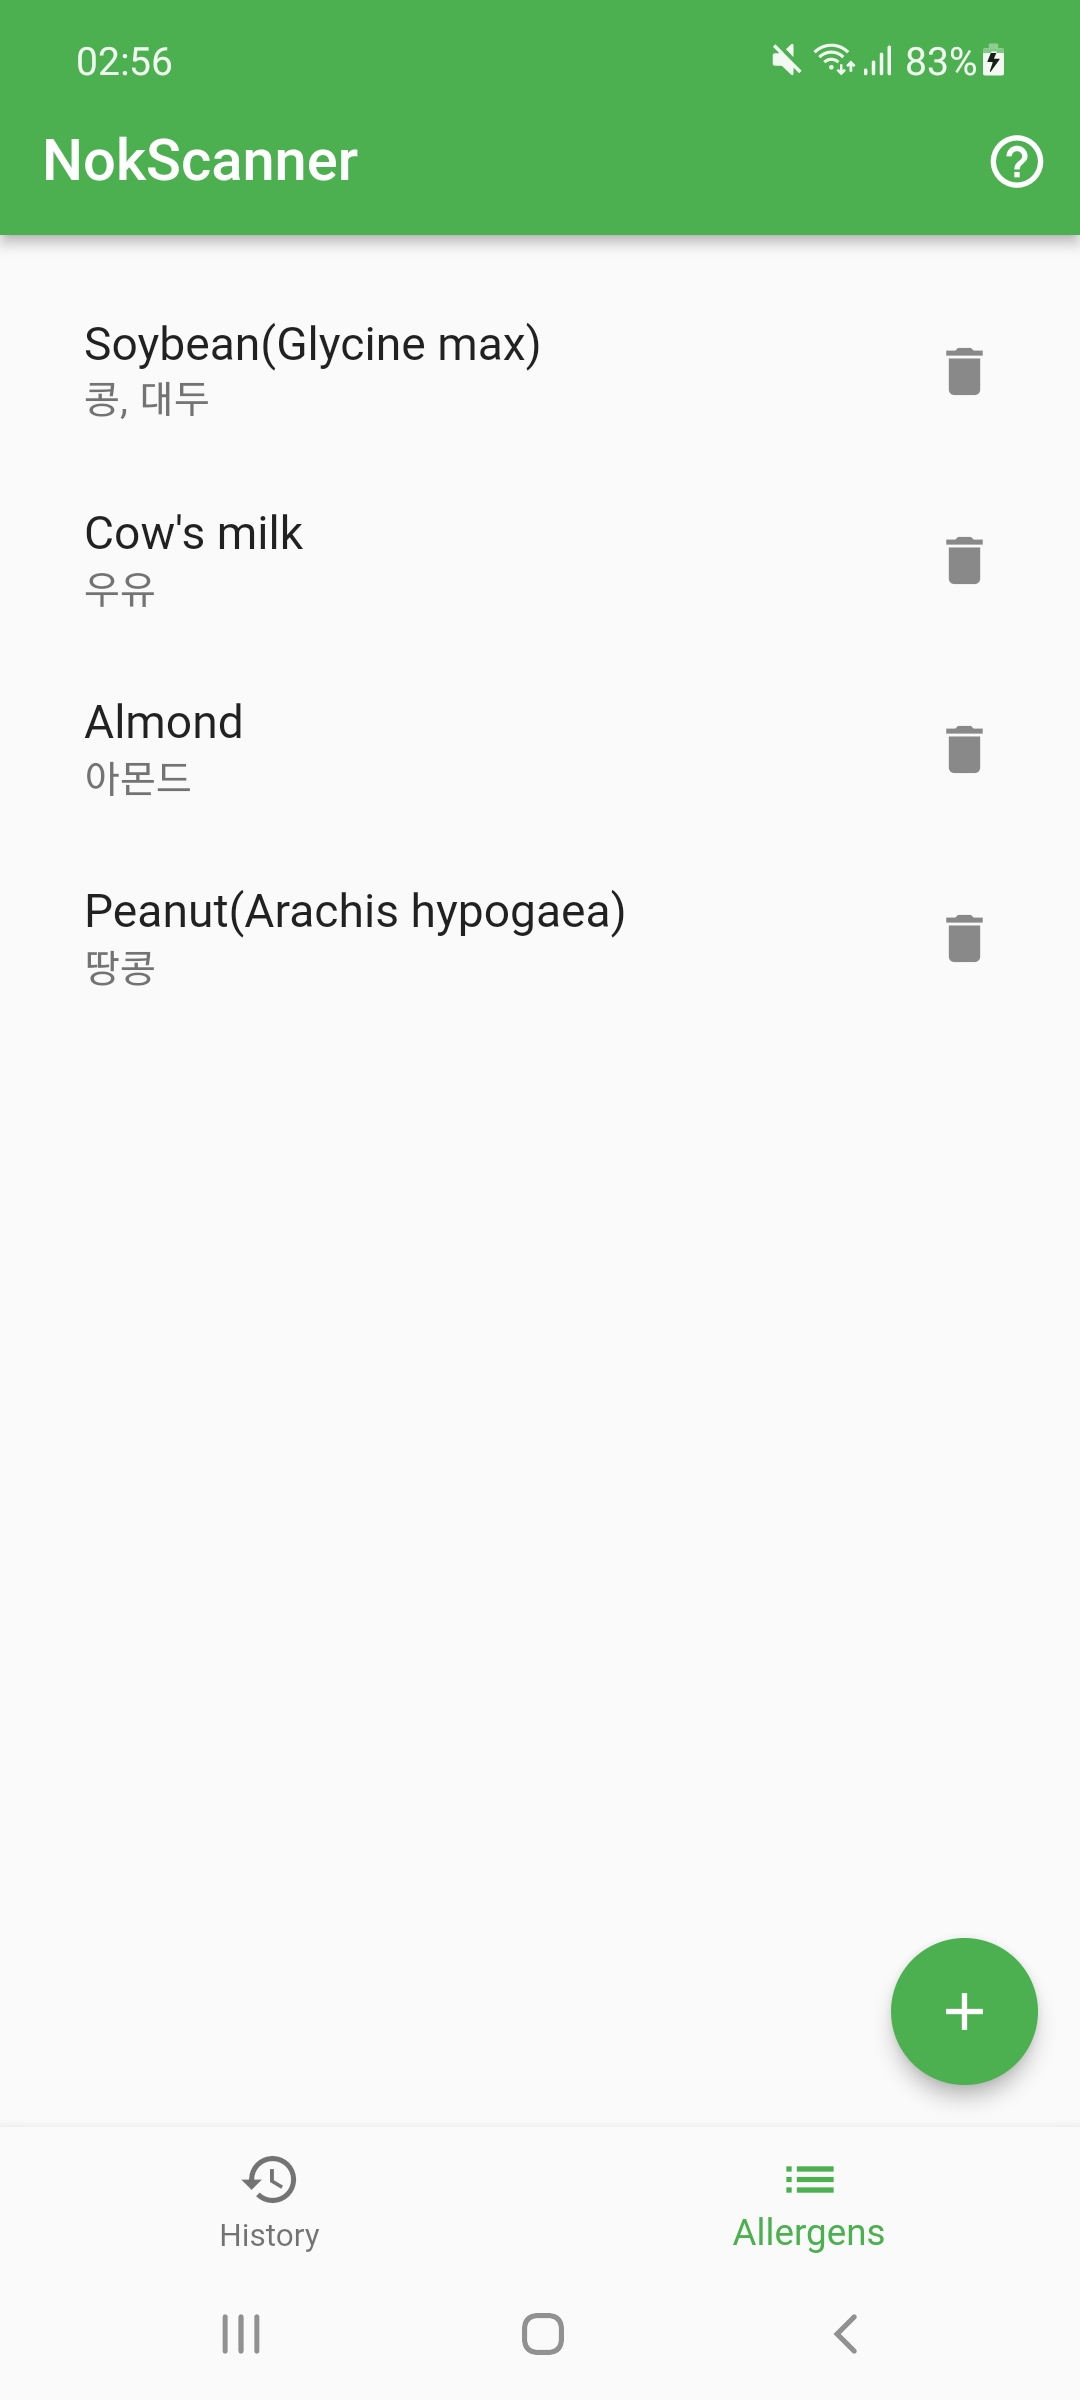
\includegraphics[width=0.5\textwidth]{Figures/Screenshot/ingredients.jpg}
  \caption{%
    Allergens screen
  }
  \label{fig:ingredients}
\end{figure}

\clearpage

When tapping the add button on the bottom right, the user can add a new unwanted ingredient to filter when scanning a product. When typing the English name, suggestions from the pre-built ingredients database are shown (Figure \ref{fig:ingredients-autocomplete}). If any of these is selected, the Korean name is autocompleted too (Figure \ref{fig:ingredients-add}). If not, the Korean name field will be guessed using the translation API. In any case, the user can manually modify both fields and press the save button on the top right to add the ingredient.

\begin{figure}[h]
    \begin{subfigure}{0.5\textwidth}
        \centering
        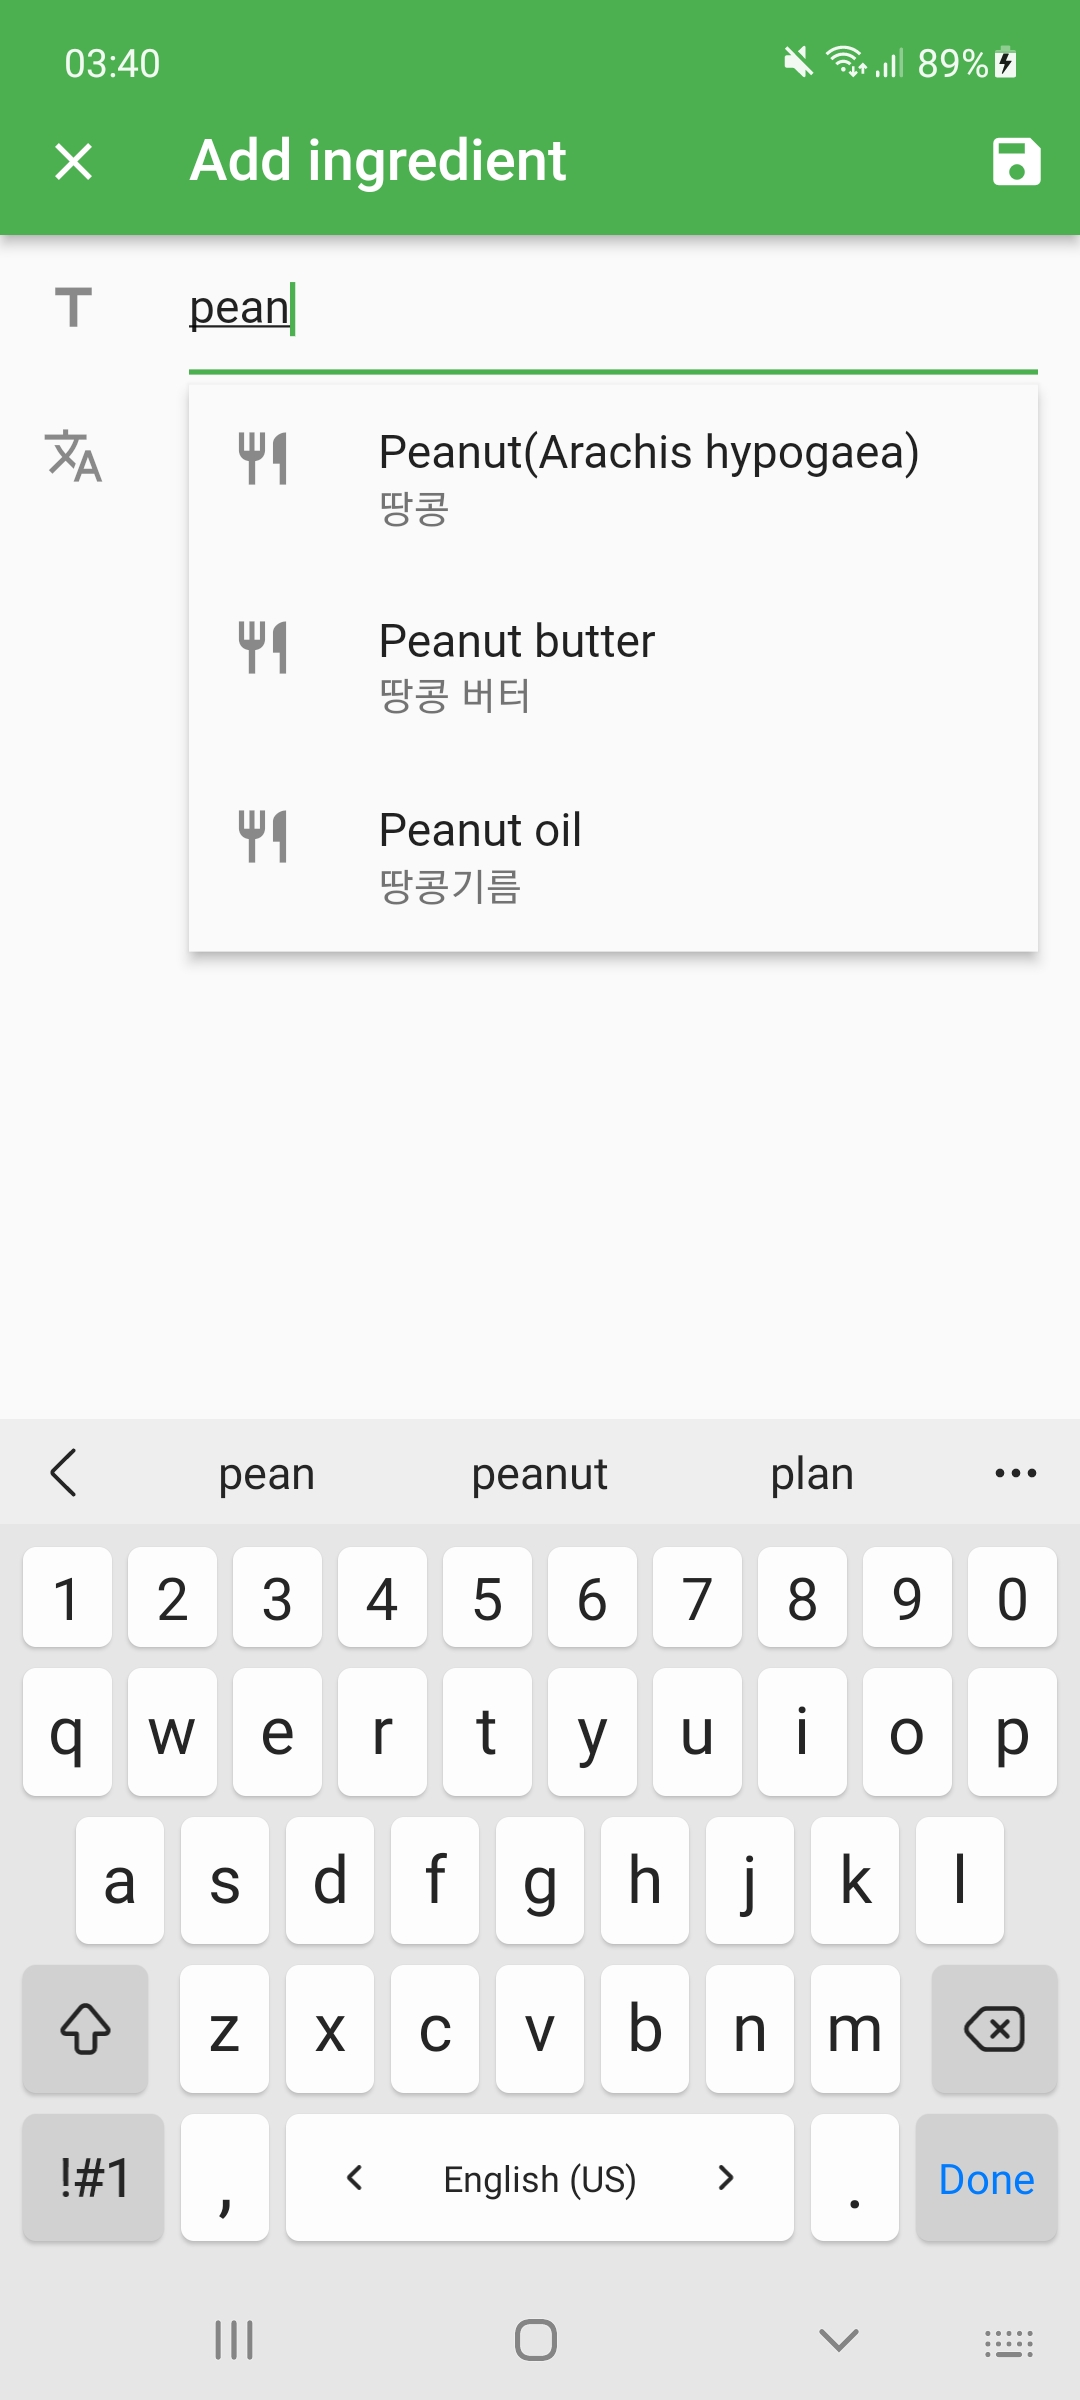
\includegraphics[width=0.9\linewidth]{Figures/Screenshot/ingredients_autocomplete.jpg} 
        \caption{Ingredient suggestions}
        \label{fig:ingredients-autocomplete}
    \end{subfigure}
    \begin{subfigure}{0.5\textwidth}
        \centering
        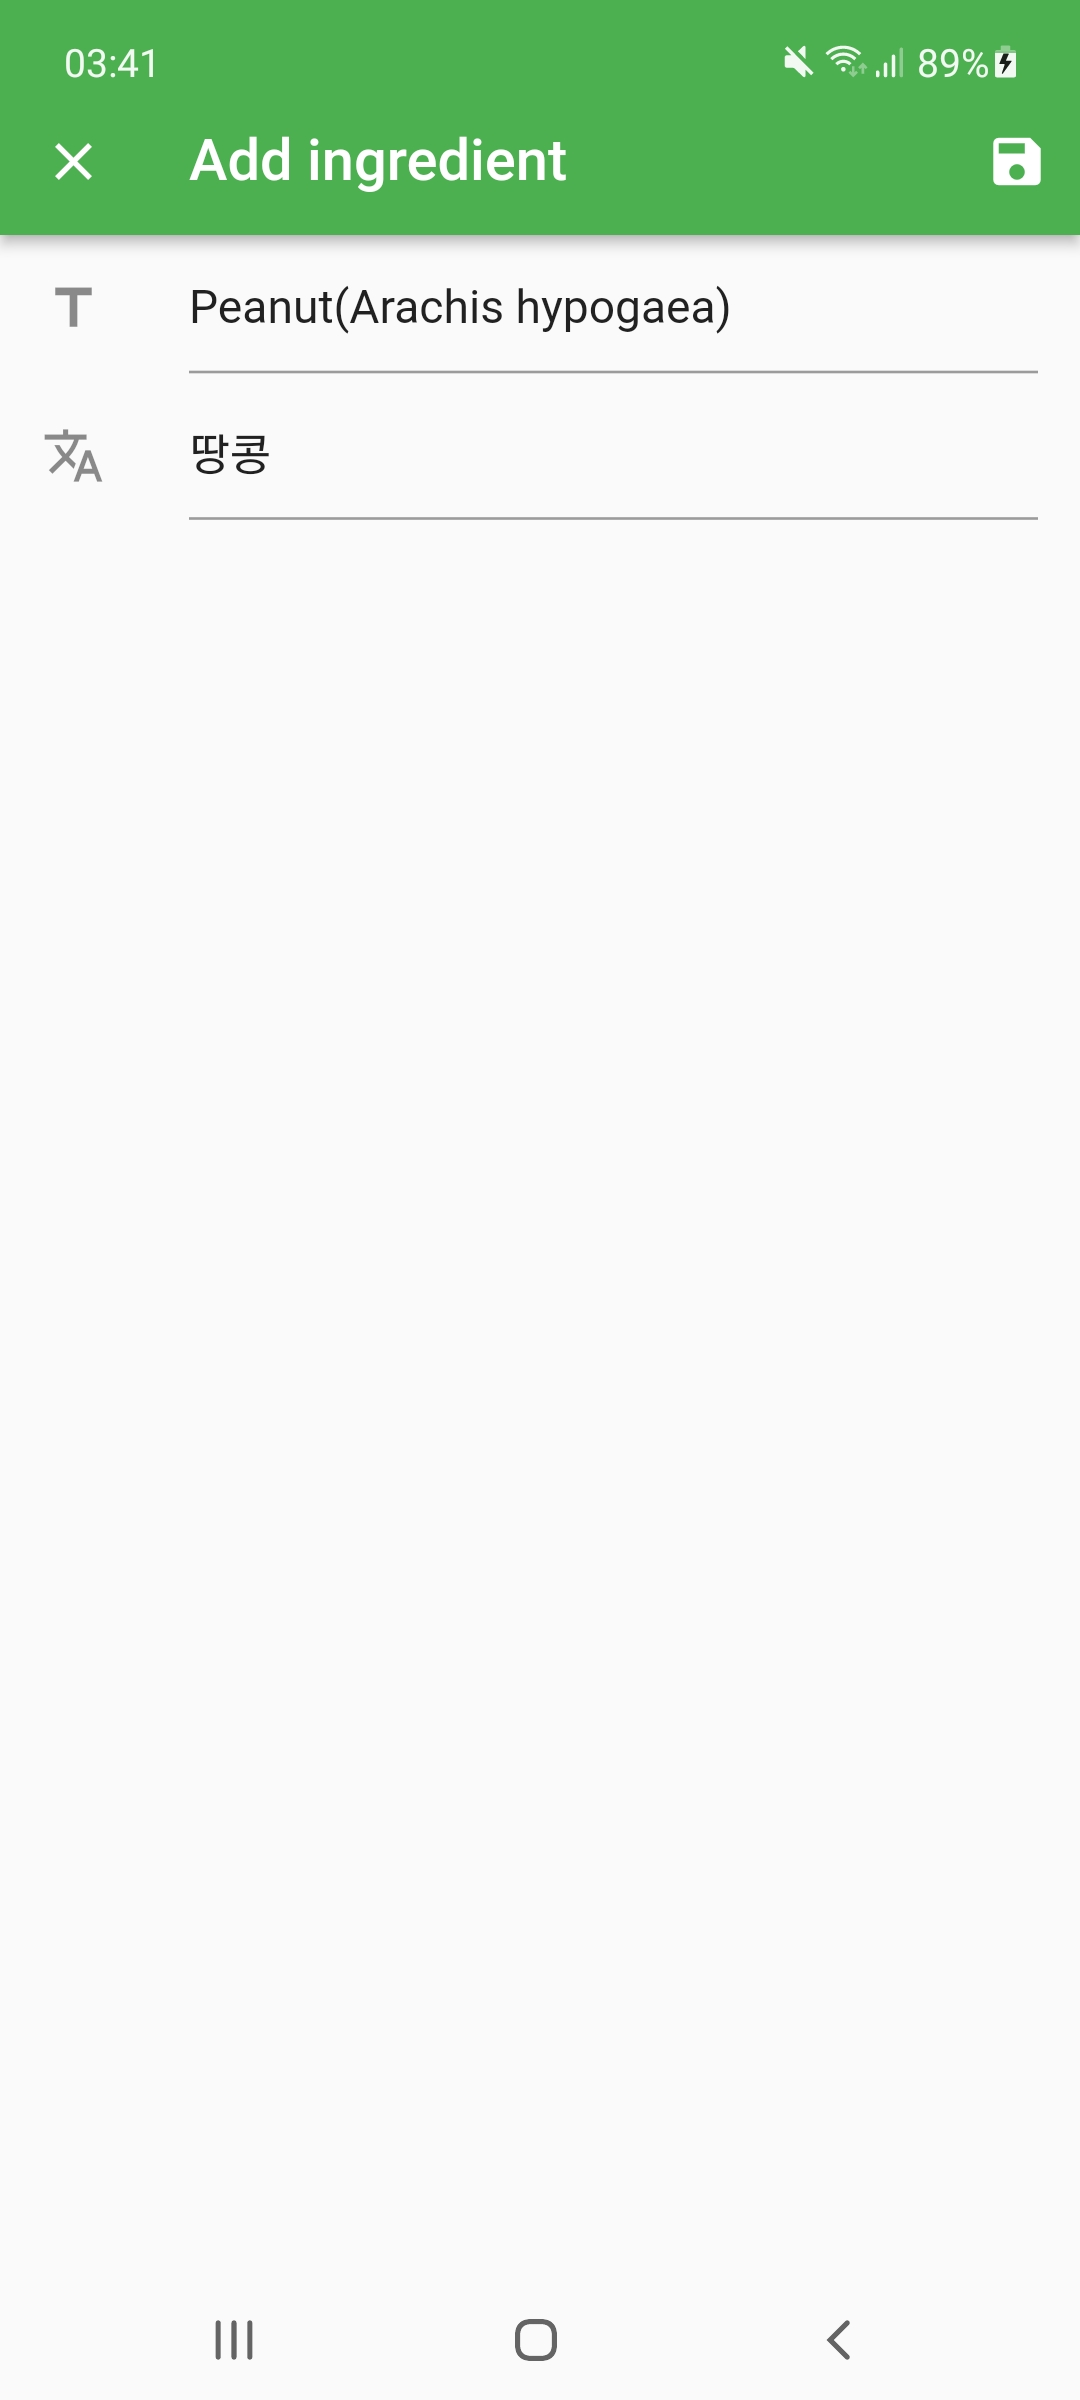
\includegraphics[width=0.9\linewidth]{Figures/Screenshot/ingredients_add.jpg}
        \caption{Autocompleted fields}
        \label{fig:ingredients-add}
    \end{subfigure}
    \caption{Add ingredient screen}
    \label{fig:ingredients2}
\end{figure}

\clearpage